\documentclass[14pt, a4paper]{article}
\usepackage[utf8]{inputenc}
\usepackage{geometry}
\usepackage{caption}
\geometry{left=2.5cm, right=2.5cm, top=2.5cm, bottom=2.5cm}
\usepackage{enumitem}
\usepackage{multicol}
\usepackage{libertinus}
\usepackage{amsmath} % Required for \text{} in math environments
\usepackage{tikz}
\usetikzlibrary{calc,angles,quotes}
\DeclareMathOperator{\arccosh}{arccosh}
\DeclareMathOperator{\arcsinh}{arcsinh}

\title{\textbf{Gilbert Strang - A First Course in Calculus} \\ \Large Chapters 1 - 7}
\author{}
\date{}

\begin{document}
\bfseries
\maketitle
\vspace{-2.5cm}

\section{Chapter 1: Introduction to Vectors}

\subsection{Vectors and Linear Combinations}
\noindent Problems 1-9 are about addition of vectors and linear combinations. 

\begin{enumerate}
    \item Describe geometrically (line, plane, or all of $R^3$) all linear combinations of
    \begin{enumerate}
        \begin{multicols}{3}
            \item $\begin{bmatrix} 1 \\ 2 \\ 3 \end{bmatrix} and \begin{bmatrix} 3 \\ 6 \\ 9 \end{bmatrix}$
            \item $\begin{bmatrix} 1 \\ 0 \\ 0 \end{bmatrix} and \begin{bmatrix} 0 \\ 2 \\ 3 \end{bmatrix}$
            \item $\begin{bmatrix} 2 \\ 0 \\ 0 \end{bmatrix} and \begin{bmatrix} 0 \\ 2 \\ 2 \end{bmatrix} and \begin{bmatrix} 2 \\ 2 \\ 3 \end{bmatrix}$
        \end{multicols}  
    \end{enumerate}  
    \item Draw $\boldsymbol{v}=\begin{bmatrix} 4 \\ 1 \end{bmatrix}$ and $\boldsymbol{w}=\begin{bmatrix} -2\\ 2 \end{bmatrix} $ and $\boldsymbol{v}+\boldsymbol{w}$ and $\boldsymbol{v}-\boldsymbol{w}$ in a single $xy$ plane.   
    \item If $\boldsymbol{v} + \boldsymbol{w} = \begin{bmatrix} 5 \\ 1 \end{bmatrix}$ and $\boldsymbol{v} - \boldsymbol{w} = \begin{bmatrix} 1 \\ 5 \end{bmatrix}$, compute and draw the vectors $\boldsymbol{v}$ and $\boldsymbol{w}$.
    \item From $\boldsymbol{v} = \begin{bmatrix} 2 \\ 1 \end{bmatrix}$ and $\boldsymbol{w} = \begin{bmatrix} 1 \\ 2 \end{bmatrix}$, find the components of $3\boldsymbol{v} + \boldsymbol{w}$ and $c\boldsymbol{v} + d\boldsymbol{w}$.
    \item Compute $\boldsymbol{u} + \boldsymbol{v} + \boldsymbol{w}$ and $2\boldsymbol{u} + 2\boldsymbol{v} + \boldsymbol{w}$. How do you know $\boldsymbol{u}, \boldsymbol{v}, \boldsymbol{w}$ lie in a plane?
    \begin{multicols}{3}
        These lie in a plane because 
        \\$\boldsymbol{w} = c\boldsymbol{u} + d\boldsymbol{v}$. Find $c$ and $d$
        \columnbreak 
        $$
        \boldsymbol{u} = \begin{bmatrix} 1 \\ 2 \\ 3 \end{bmatrix}, \quad \boldsymbol{v} = \begin{bmatrix} -3 \\ 1 \\ -2 \end{bmatrix}, \quad \boldsymbol{w} = \begin{bmatrix} 2 \\ -3 \\ -1 \end{bmatrix}.
        $$
    \end{multicols}
    \item Every combination of $\boldsymbol{v} = (1, -2, 1)$ and $\boldsymbol{w} = (0, 1, -1)$ has components that add to \underline{\hspace{1cm}}.
    \\Find $c$ and $d$ so that $c\boldsymbol{v} + d\boldsymbol{w} = (3, 3, -6)$. Why is $(3, 3, 6)$ impossible?

    \item In the $xy$ plane mark all nine of these linear combinations:
    $$
    c\begin{bmatrix} 2 \\ 1 \end{bmatrix} + d\begin{bmatrix} 0 \\ 1 \end{bmatrix} \quad \text{with} \quad c = 0,1,2 \quad \text{and} \quad d = 0,1,2.
    $$

    \item The parallelogram in Figure 1.1 has diagonal $\boldsymbol{v} + \boldsymbol{w}$. What is its other diagonal? What is the sum of the two diagonals? Draw that vector sum.

    \item If three corners of a parallelogram are $(1,1), (4,2)$, and $(1,3)$, what are all three of the possible fourth corners? Draw two of them.
\end{enumerate}

\noindent Problems 10--14 are about special vectors on cubes and clocks in Figure 1.4.

\begin{enumerate}[resume]
    \item Which point of the cube is $\boldsymbol{i} + \boldsymbol{j}$? Which point is the vector sum of $\boldsymbol{i} = (1,0,0)$ and $\boldsymbol{j} = (0,1,0)$ and $\boldsymbol{k} = (0,0,1)$? Describe all points $(x,y,z)$ in the cube.

    \item Four corners of this unit cube are $(0,0,0), (1,0,0), (0,1,0), (0,0,1)$. What are the other four corners? Find the coordinates of the center point of the cube. The center points of the six faces are \underline{\hspace{2cm}}. The cube has how many edges?

    \item Review Question. In $xyz$ space, where is the plane of all linear combinations of $\boldsymbol{i} = (1,0,0)$ and $\boldsymbol{i} + \boldsymbol{j} = (1,1,0)$?
    \newpage
    \item 
    \begin{enumerate}
        \item What is the sum $V$ of the twelve vectors that go from the center of a clock to the hours 1:00, 2:00, \dots, 12:00?
        \item If the 2:00 vector is removed, why do the 11 remaining vectors add to 8:00?
        \item What are the $x, y$ components of that 2:00 vector $\boldsymbol{v} = (\cos\theta, \sin\theta)$?
    \end{enumerate}
    \item Suppose the twelve vectors start from 6:00 at the bottom instead of $(0,0)$ at the center. The vector to 12:00 is doubled to $(0,2)$. The new twelve vectors add to \underline{\hspace{2cm}}.
\end{enumerate}

    \begin{figure}[htbp] % figure 环境用于浮动体，[htbp] 尝试指定位置偏好
        \centering % 图片居中
        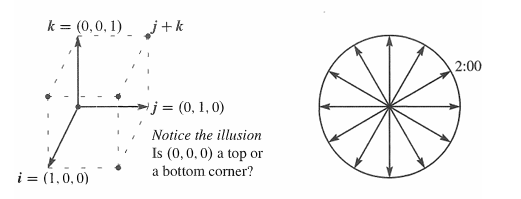
\includegraphics[width=0.8\textwidth]{pic/Figure1.4.png} % 插入图片，指定宽度为文本宽度的 80%
        \renewcommand{\thefigure}{1.4}% 强行将当前的图片编号改为 1.4
        \caption{ Unit cube from i,j, k and twelve clock vectors.}
        %\label{fig:my_label} % 标签，用于交叉引用（可选）
    \end{figure}

\noindent Problems 15--19 go further with linear combinations of $\boldsymbol{v}$ and $\boldsymbol{w}$ (Figure 1.5a).

\begin{enumerate}[resume]

    \item Figure 1.5a shows $\frac{1}{2}\,\boldsymbol{v} + \frac{1}{2}\,\boldsymbol{w}$. Mark the points $\frac{3}{4}\,\boldsymbol{v} + \frac{1}{4}\,\boldsymbol{w}$ and $\frac{1}{4}\,\boldsymbol{v} + \frac{3}{4}\,\boldsymbol{w}$ and $\boldsymbol{v} + \boldsymbol{w}$.

    \item Mark the point $-\boldsymbol{v} + 2\boldsymbol{w}$ and any other combination $c\boldsymbol{v} + d\boldsymbol{w}$ with $c + d = 1$. Draw the line of all combinations that have $c + d = 1$.

    \item Locate $\frac{1}{3}\,\boldsymbol{v} + \frac{1}{3}\,\boldsymbol{w}$ and $\frac{2}{3}\,\boldsymbol{v} + \frac{2}{3}\,\boldsymbol{w}$. The combinations $c\boldsymbol{v} + c\boldsymbol{w}$ fill out what line?

    \item Restricted by $0 \le c \le 1$ and $0 \le d \le 1$, shade in all combinations $c\boldsymbol{v} + d\boldsymbol{w}$.

    \item Restricted only by $c \ge 0$ and $d \ge 0$ draw the ``cone'' of all combinations $c\boldsymbol{v} + d\boldsymbol{w}$. 
\end{enumerate}

    \begin{figure}[htbp] % figure 环境用于浮动体，[htbp] 尝试指定位置偏好
        \centering % 图片居中
        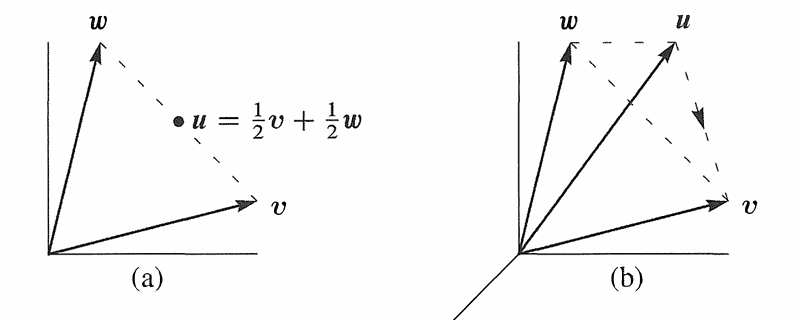
\includegraphics[width=0.8\textwidth]{pic/Figure1.5.png} % 插入图片，指定宽度为文本宽度的 80%
        \renewcommand{\thefigure}{1.5}% 强行将当前的图片编号改为 1.5
        \caption{  Problems 15-19 in a plane \quad\quad\quad\quad  Problems 20-25 in 3-dimensional space}
        \label{fig:my_label} % 标签，用于交叉引用（可选）
    \end{figure}

\noindent Problems 20-25 deal with $u$, $v$, $w$ in three-dimensional space (see Figure 1.5b). 

\begin{enumerate}[resume]
    \item Locate $\frac{1}{2}\,\boldsymbol{v} + \frac{1}{2}\,\boldsymbol{w} + \frac{1}{2}\,\boldsymbol{v}$ and $\frac{1}{2}\,\boldsymbol{v} + \frac{1}{2}\,\boldsymbol{w} + \frac{1}{2}\,\boldsymbol{w}$ in Figure 1.5b. Challenge problem: Under what restrictions on $c, d, e$, will the combinations $c\boldsymbol{u} + d\boldsymbol{v} + e\boldsymbol{w}$ fill in the dashed triangle? To stay in the triangle, one requirement is $c \ge 0, d \ge 0, e \ge 0$.

    \item The three sides of the dashed triangle are $\boldsymbol{v} - \boldsymbol{u}$ and $\boldsymbol{w} - \boldsymbol{v}$ and $\boldsymbol{u} - \boldsymbol{w}$. Their sum is \underline{\hspace{2cm}}. Draw the head-to-tail addition around a plane triangle of $(3,1)$ plus $(-1,1)$ plus $(-2,-2)$.

    \item Shade in the pyramid of combinations $c\boldsymbol{u} + d\boldsymbol{v} + e\boldsymbol{w}$ with $c \ge 0$, $d \ge 0$, $e \ge 0$ and $c + d + e \le 1$. Mark the vector $\frac{1}{2}(\boldsymbol{u} + \boldsymbol{v} + \boldsymbol{w})$ as inside or outside this pyramid.

    \item If you look at all combinations of those $\boldsymbol{u}, \boldsymbol{v},$ and $\boldsymbol{w}$, is there any vector that can't be produced from $c\boldsymbol{u} + d\boldsymbol{v} + e\boldsymbol{w}$? Different answer if $\boldsymbol{u}, \boldsymbol{v}, \boldsymbol{w}$ are all in \underline{\hspace{2cm}}.

    \item Which vectors are combinations of $\boldsymbol{u}$ and $\boldsymbol{v}$, and also combinations of $\boldsymbol{v}$ and $\boldsymbol{w}$?

    \item Draw vectors $\boldsymbol{u}, \boldsymbol{v}, \boldsymbol{w}$ so that their combinations $c\boldsymbol{u} + d\boldsymbol{v} + e\boldsymbol{w}$ fill only a line. Find vectors $\boldsymbol{u}, \boldsymbol{v}, \boldsymbol{w}$ so that their combinations $c\boldsymbol{u} + d\boldsymbol{v} + e\boldsymbol{w}$ fill only a plane.

    \item What combination $c\begin{bmatrix} 2 \\ 1 \end{bmatrix} + d\begin{bmatrix} 3 \\ 1 \end{bmatrix}$ produces $\begin{bmatrix} 14 \\ 8 \end{bmatrix}$? Express this question as two equations for the coefficients $c$ and $d$ in the linear combination.
\end{enumerate}


\paragraph{Challenge Problems}
\begin{enumerate}[resume]
    \item How many corners does a cube have in 4 dimensions? How many 3D faces? How many edges? A typical corner is $(0,0,1,0)$. A typical edge goes to $(0,1,0,0)$.

    \item Find vectors $\boldsymbol{v}$ and $\boldsymbol{w}$ so that $\boldsymbol{v} + \boldsymbol{w} = (4,5,6)$ and $\boldsymbol{v} - \boldsymbol{w} = (2,5,8)$. This is a question with \underline{\hspace{2cm}} unknown numbers, and an equal number of equations to find those numbers.

    \item Find two different combinations of the three vectors $\boldsymbol{u} = (1,3)$ and $\boldsymbol{v} = (2,7)$ and $\boldsymbol{w} = (1,5)$ that produce $\boldsymbol{b} = (0,1)$. Slightly delicate question: If I take any three vectors $\boldsymbol{u}, \boldsymbol{v}, \boldsymbol{w}$ in the plane, will there always be two different combinations that produce $\boldsymbol{b} = (0,1)$?

    \item The linear combinations of $\boldsymbol{v} = (a,b)$ and $\boldsymbol{w} = (c,d)$ fill the plane unless \underline{\hspace{2cm}}. \\Find four vectors $\boldsymbol{u}, \boldsymbol{v}, \boldsymbol{w}, \boldsymbol{z}$ with four components each so that their combinations $c\boldsymbol{u} + d\boldsymbol{v} + e\boldsymbol{w} + f\boldsymbol{z}$ produce all vectors $(b_1, b_2, b_3, b_4)$ in four-dimensional space.

    \item Write down three equations for $c, d, e$ so that $c\boldsymbol{u} + d\boldsymbol{v} + e\boldsymbol{w} = \boldsymbol{b}$. Can you somehow find $c, d, e$ for $\boldsymbol{b}$?
    \[
    \boldsymbol{u} = \begin{bmatrix} 2 \\ -1 \\ 0 \end{bmatrix}, \quad
    \boldsymbol{v} = \begin{bmatrix} -1 \\ 2 \\ -1 \end{bmatrix}, \quad
    \boldsymbol{w} = \begin{bmatrix} 0 \\ -1 \\ 2 \end{bmatrix}, \quad
    \boldsymbol{b} = \begin{bmatrix} 1 \\ 0 \\ 0 \end{bmatrix}.
    \]
\end{enumerate}

\subsection{Lengths and Dot Products}
\begin{enumerate}
    \item Calculate the dot products $\boldsymbol{u} \cdot \boldsymbol{v}$ and $\boldsymbol{u} \cdot \boldsymbol{w}$ and $\boldsymbol{u} \cdot (\boldsymbol{v} + \boldsymbol{w})$ and $\boldsymbol{w} \cdot \boldsymbol{v}$:
    \[
    \boldsymbol{u} = \begin{bmatrix} -.6 \\ .8 \end{bmatrix}, \qquad
    \boldsymbol{v} = \begin{bmatrix} 4 \\ 3 \end{bmatrix}, \qquad
    \boldsymbol{w} = \begin{bmatrix} 1 \\ 2 \end{bmatrix}.
    \]

    \item Compute the lengths $\|\boldsymbol{u}\|$ and $\|\boldsymbol{v}\|$ and $\|\boldsymbol{w}\|$ of those vectors. Check the Schwarz inequalities $|\boldsymbol{u} \cdot \boldsymbol{v}| \le \|\boldsymbol{u}\| \, \|\boldsymbol{v}\|$ and $\boldsymbol{v} \cdot \boldsymbol{w} \le \|\boldsymbol{v}\| \, \|\boldsymbol{w}\|$.

    \item Find unit vectors in the directions of $\boldsymbol{v}$ and $\boldsymbol{w}$ in Problem 1, and the cosine of the angle $\theta$. Choose vectors $\boldsymbol{a}, \boldsymbol{b}, \boldsymbol{c}$ that make $0^\circ$, $90^\circ$, and $180^\circ$ angles with $\boldsymbol{w}$.

    \item For any \emph{unit} vectors $\boldsymbol{v}$ and $\boldsymbol{w}$, find the dot products (actual numbers) of  
    \begin{enumerate}
        \begin{multicols}{3}
            \item $\boldsymbol{v}$ and $-\boldsymbol{v}$  
            \item $\boldsymbol{v} + \boldsymbol{w}$ and $\boldsymbol{v} - \boldsymbol{w}$  
            \item $\boldsymbol{v} - 2\boldsymbol{w}$ and $\boldsymbol{v} + 2\boldsymbol{w}$
        \end{multicols}
    \end{enumerate}

    \item Find unit vectors $\boldsymbol{u}_1$ and $\boldsymbol{u}_2$ in the directions of $\boldsymbol{v} = (1,3)$ and $\boldsymbol{w} = (2,1,2)$. Find unit vectors $\boldsymbol{U}_1$ and $\boldsymbol{U}_2$ that are perpendicular to $\boldsymbol{u}_1$ and $\boldsymbol{u}_2$.

    \item 
    \begin{enumerate}
        \item Describe every vector $\boldsymbol{w} = (w_1, w_2)$ that is perpendicular to $\boldsymbol{v} = (2, -1)$.
        \item All vectors perpendicular to $\boldsymbol{V} = (1,1,1)$ lie on a \underline{\hspace{2cm}} in 3 dimensions.
        \item The vectors perpendicular to both $(1,1,1)$ and $(1,2,3)$ lie on a \underline{\hspace{2cm}}.
    \end{enumerate}

    \item Find the angle $\theta$ (from its cosine) between these pairs of vectors:
    \begin{enumerate}
        \begin{multicols}{2}
            \item $\displaystyle \boldsymbol{v} = \begin{bmatrix} 1 \\ \sqrt{3} \end{bmatrix}$ and $\displaystyle \boldsymbol{w} = \begin{bmatrix} 1 \\ 0 \end{bmatrix}$
            \item $\displaystyle \boldsymbol{v} = \begin{bmatrix} 2 \\ 2 \\ -1 \end{bmatrix}$ and $\displaystyle \boldsymbol{w} = \begin{bmatrix} 2 \\ -1 \\ 2 \end{bmatrix}$
        \end{multicols}
        \begin{multicols}{2}
            \item $\displaystyle \boldsymbol{v} = \begin{bmatrix} 1 \\ \sqrt{3} \end{bmatrix}$ and $\displaystyle \boldsymbol{w} = \begin{bmatrix} -1 \\ \sqrt{3} \end{bmatrix}$
            \item $\displaystyle \boldsymbol{v} = \begin{bmatrix} 3 \\ 1 \end{bmatrix}$ and $\displaystyle \boldsymbol{w} = \begin{bmatrix} -1 \\ -2 \end{bmatrix}$
        \end{multicols}
    \end{enumerate}

    \item True or false (give a reason if true or find a counterexample if false):
    \begin{enumerate}
        \item If $\boldsymbol{u} = (1,1,1)$ is perpendicular to $\boldsymbol{v}$ and $\boldsymbol{w}$, then $\boldsymbol{v}$ is parallel to $\boldsymbol{w}$.
        \item If $\boldsymbol{u}$ is perpendicular to $\boldsymbol{v}$ and $\boldsymbol{w}$, then $\boldsymbol{u}$ is perpendicular to $\boldsymbol{v} + 2\boldsymbol{w}$.
        \item If $\boldsymbol{u}$ and $\boldsymbol{v}$ are perpendicular unit vectors then $\|\boldsymbol{u} - \boldsymbol{v}\| = \sqrt{2}$. Yes!
    \end{enumerate}

    \item The slopes of the arrows from $(0,0)$ to $(v_1,v_2)$ and $(w_1,w_2)$ are $v_2/v_1$ and $w_2/w_1$. Suppose the product $v_2 w_2 / v_1 w_1$ of those slopes is $-1$. Show that $\boldsymbol{v} \cdot \boldsymbol{w} = 0$ and the vectors are perpendicular. (The line $y = 4x$ is perpendicular to $y = -\frac{1}{4}x$.)

    \item Draw arrows from $(0,0)$ to the points $\boldsymbol{v} = (1,2)$ and $\boldsymbol{w} = (-2,1)$. Multiply their slopes. That answer is a signal that $\boldsymbol{v} \cdot \boldsymbol{w} = 0$ and the arrows are \underline{\hspace{2cm}}.

    \item If $\boldsymbol{v} \cdot \boldsymbol{w}$ is negative, what does this say about the angle between $\boldsymbol{v}$ and $\boldsymbol{w}$? Draw a 3-dimensional vector $\boldsymbol{v}$ (an arrow), and show where to find all $\boldsymbol{w}$'s with $\boldsymbol{v} \cdot \boldsymbol{w} < 0$.

    \item With $\boldsymbol{v} = (1,1)$ and $\boldsymbol{w} = (1,5)$ choose a number $c$ so that $\boldsymbol{w} - c\boldsymbol{v}$ is perpendicular to $\boldsymbol{v}$. Then find the formula for $c$ starting from any nonzero $\boldsymbol{v}$ and $\boldsymbol{w}$.

    \item Find nonzero vectors $\boldsymbol{v}$ and $\boldsymbol{w}$ that are perpendicular to $(1,0,1)$ and to each other.

    \item Find nonzero vectors $\boldsymbol{u}, \boldsymbol{v}, \boldsymbol{w}$ that are perpendicular to $(1,1,1)$ and to each other.

    \item The geometric mean of $x = 2$ and $y = 8$ is $\sqrt{xy} = 4$. The arithmetic mean is larger: $\frac{1}{2}(x + y) = \underline{\hspace{2cm}}$. This would come in Example 6 from the Schwarz inequality for $\boldsymbol{v} = (\sqrt{2}, \sqrt{8})$ and $\boldsymbol{w} = (\sqrt{8}, \sqrt{2})$. Find $\cos\theta$ for this $\boldsymbol{v}$ and $\boldsymbol{w}$.

    \item How long is the vector $\boldsymbol{v} = (1,1,\dots,1)$ in 9 dimensions? Find a unit vector $\boldsymbol{u}$ in the same direction as $\boldsymbol{v}$ and a unit vector $\boldsymbol{w}$ that is perpendicular to $\boldsymbol{v}$.

    \item What are the cosines of the angles $\alpha, \beta, \theta$ between the vector $(1,0,-1)$ and the unit vectors $\boldsymbol{i}, \boldsymbol{j}, \boldsymbol{k}$ along the axes? Check the formula $\cos^2\alpha + \cos^2\beta + \cos^2\theta = 1$.
\end{enumerate}

\noindent Problems 18-28 lead to the main facts about lengths and angles in triangles. 
\begin{enumerate}[resume]
    \item The parallelogram with sides $\boldsymbol{v} = (4,2)$ and $\boldsymbol{w} = (-1,2)$ is a rectangle. Check the Pythagoras formula $a^2 + b^2 = c^2$ which is for \emph{right triangles only}:
    \[
    \boxed{(\text{length of } \boldsymbol{v})^2 + (\text{length of } \boldsymbol{w})^2 = (\text{length of } \boldsymbol{v} + \boldsymbol{w})^2.}
    \]

    \item (Rules for dot products) These equations are simple but useful:
    \begin{enumerate}
        \begin{multicols}{3}
            \item $\boldsymbol{v} \cdot \boldsymbol{w} = \boldsymbol{w} \cdot \boldsymbol{v}$
            \item $\boldsymbol{u} \cdot (\boldsymbol{v} + \boldsymbol{w}) = \boldsymbol{u} \cdot \boldsymbol{v} + \boldsymbol{u} \cdot \boldsymbol{w}$
            \item $(c\boldsymbol{v}) \cdot \boldsymbol{w} = c(\boldsymbol{v} \cdot \boldsymbol{w})$    
        \end{multicols}
    \end{enumerate}
    Use (2) with $\boldsymbol{u} = \boldsymbol{v} + \boldsymbol{w}$ to prove 
    $\|\boldsymbol{v} + \boldsymbol{w}\|^2 = \boldsymbol{v} \cdot \boldsymbol{v} + 2\boldsymbol{v} \cdot \boldsymbol{w} + \boldsymbol{w} \cdot \boldsymbol{w}.$

    \item The ``Law of Cosines'' comes from $(\boldsymbol{v} - \boldsymbol{w}) \cdot (\boldsymbol{v} - \boldsymbol{w}) = \boldsymbol{v} \cdot \boldsymbol{v} - 2\boldsymbol{v} \cdot \boldsymbol{w} + \boldsymbol{w} \cdot \boldsymbol{w}$:
    \[
    \textbf{Cosine Law} \qquad \|\boldsymbol{v} - \boldsymbol{w}\|^2 = \|\boldsymbol{v}\|^2 - 2\|\boldsymbol{v}\|\,\|\boldsymbol{w}\|\cos\theta + \|\boldsymbol{w}\|^2.
    \]
    Draw a triangle with sides $\boldsymbol{v}$ and $\boldsymbol{w}$ and $\boldsymbol{v} - \boldsymbol{w}$. Which of the angles is $\theta$?
    \newpage
    \item The \textbf{triangle inequality} says: (length of $\boldsymbol{v} + \boldsymbol{w}$) $\le$ (length of $\boldsymbol{v}$) + (length of $\boldsymbol{w}$).  
    \\Problem 19 found $\|\boldsymbol{v} + \boldsymbol{w}\|^2 = \|\boldsymbol{v}\|^2 + 2\boldsymbol{v} \cdot \boldsymbol{w} + \|\boldsymbol{w}\|^2$. 
    \\Increase by $\|\boldsymbol{v}\|\,\|\boldsymbol{w}\|$ to show that $\boldsymbol{v} \cdot \boldsymbol{w}$ can not exceed $\|\boldsymbol{v}\|\,\|\boldsymbol{w}\|$:  
    \begin{multicols}{4}
        \textbf{Triangle inequality}
        \columnbreak
        $$
        \|\boldsymbol{v} + \boldsymbol{w}\|^2 \le (\|\boldsymbol{v}\| + \|\boldsymbol{w}\|)^2 
        \quad \text{or} \quad 
        \boxed{\|\boldsymbol{v} + \boldsymbol{w}\| \le \|\boldsymbol{v}\| + \|\boldsymbol{w}\|}.
        $$
    \end{multicols}
    \begin{figure}[htbp] % figure 环境用于浮动体，[htbp] 尝试指定位置偏好
        \centering % 图片居中
        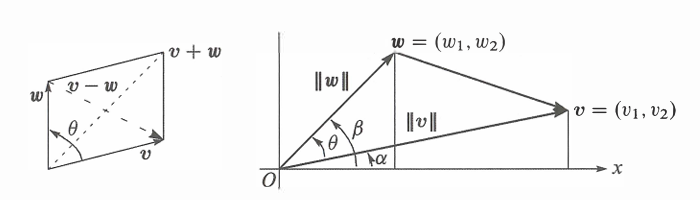
\includegraphics[width=0.8\textwidth]{pic/Figure_21.png} % 插入图片，指定宽度为文本宽度的 80%
        %\renewcommand{\thefigure}{1.5}% 强行将当前的图片编号改为 1.5
        %\caption{ }%标题
        %\label{fig:my_label} % 标签，用于交叉引用（可选）
    \end{figure}

    \item The Schwarz inequality $|\boldsymbol{v} \cdot \boldsymbol{w}| \le \|\boldsymbol{v}\| \, \|\boldsymbol{w}\|$ by algebra instead of trigonometry:
    \begin{enumerate}
        \item Multiply out both sides of $(v_1 w_1 + v_2 w_2)^2 \le (v_1^2 + v_2^2)(w_1^2 + w_2^2)$.
        \item Show that the difference between those two sides equals $(v_1 w_2 - v_2 w_1)^2$. This cannot be negative since it is a square---so the inequality is true.
    \end{enumerate}

    \item The figure shows that $\cos\alpha = v_1/\|\boldsymbol{v}\|$ and $\sin\alpha = v_2/\|\boldsymbol{v}\|$. Similarly $\cos\beta$ is \underline{\hspace{1cm}} and $\sin\beta$ is \underline{\hspace{1cm}}. The angle $\theta$ is $\beta - \alpha$. Substitute into the trigonometry formula $\cos\beta \cos\alpha + \sin\beta \sin\alpha$ for $\cos(\beta - \alpha)$ to find 
    $
    \cos\theta = \boldsymbol{v} \cdot \boldsymbol{w} / \|\boldsymbol{v}\| \, \|\boldsymbol{w}\|.
    $

    \item One-line proof of the inequality $|\boldsymbol{u} \cdot \boldsymbol{U}| \le 1$ for unit vectors $(u_1, u_2)$ and $(U_1, U_2)$:
    \[
    |\boldsymbol{u} \cdot \boldsymbol{U}| 
    \le |u_1||U_1| + |u_2||U_2| 
    \le \frac{u_1^2 + U_1^2}{2} + \frac{u_2^2 + U_2^2}{2} = 1.
    \]
    Put $(u_1, u_2) = (.6, .8)$ and $(U_1, U_2) = (.8, .6)$ in that whole line and find $\cos\theta$.

    \item Why is $|\cos\theta|$ never greater than 1 in the first place?

    \item (Recommended) Draw a parallelogram.

    \item Parallelogram with two sides $\boldsymbol{v}$ and $\boldsymbol{w}$. Show that the squared diagonal lengths $\|\boldsymbol{v} + \boldsymbol{w}\|^2 + \|\boldsymbol{v} - \boldsymbol{w}\|^2$ add to the sum of four squared side lengths $2\|\boldsymbol{v}\|^2 + 2\|\boldsymbol{w}\|^2$.

    \item If $\boldsymbol{v} = (1,2)$ draw all vectors $\boldsymbol{w} = (x,y)$ in the $xy$-plane with $\boldsymbol{v} \cdot \boldsymbol{w} = x + 2y = 5$. Why do those $\boldsymbol{w}$'s lie along a line? Which is the shortest $\boldsymbol{w}$?

    \item (Recommended) If $\|\boldsymbol{v}\| = 5$ and $\|\boldsymbol{w}\| = 3$, what are the smallest and largest possible values of $\|\boldsymbol{v} - \boldsymbol{w}\|$? What are the smallest and largest possible values of $\boldsymbol{v} \cdot \boldsymbol{w}$?
\end{enumerate}

\paragraph{Challenge Problems}
\begin{enumerate}[resume]
    \item Can three vectors in the $xy$-plane have $\boldsymbol{u} \cdot \boldsymbol{v} < 0$ and $\boldsymbol{v} \cdot \boldsymbol{w} < 0$ and $\boldsymbol{u} \cdot \boldsymbol{w} < 0$? \\
    I don't know how many vectors in $xyz$ space can have all negative dot products. (Four of those vectors in the plane would certainly be impossible\dots.)

    \item Pick any numbers that add to $x + y + z = 0$. Find the angle between your vector $\boldsymbol{v} = (x, y, z)$ and the vector $\boldsymbol{w} = (z, x, y)$. Challenge question: Explain why 
    $
    \boldsymbol{v} \cdot \boldsymbol{w} / \|\boldsymbol{v}\| \, \|\boldsymbol{w}\| \text{ is always } -\frac{1}{2}.
    $

    \item How could you prove $\sqrt[3]{xyz} \le \frac{1}{3}(x + y + z)$ (geometric mean $\le$ arithmetic mean)?

    \item Find 4 perpendicular unit vectors of the form $\left(\pm \tfrac{1}{2}, \pm \tfrac{1}{2}, \pm \tfrac{1}{2}, \pm \tfrac{1}{2}\right)$: Choose $+$ or $-$.

    \item Using $\boldsymbol{v} = \texttt{randn}(3,1)$ in MATLAB, create a random unit vector $\boldsymbol{u} = \boldsymbol{v}/\|\boldsymbol{v}\|$.
    \\ Using $\boldsymbol{V} = \texttt{randn}(3,30)$ create 30 more random unit vectors $\boldsymbol{U}_j$.
    \\ What is the average size of the dot products $|\boldsymbol{u} \cdot \boldsymbol{U}_j|$? 
    \\ In calculus, the average is $\displaystyle \int_0^\pi |\cos\theta| \,{d\theta}/{\pi} = {2}/{\pi}$.
\end{enumerate}


\subsection{Matrices}
\begin{enumerate}
    \item Find the linear combination $3\boldsymbol{s}_1 + 4\boldsymbol{s}_2 + 5\boldsymbol{s}_3 = \boldsymbol{b}$. Then write $\boldsymbol{b}$ as a matrix-vector multiplication $S\boldsymbol{x}$, with $3,4,5$ in $\boldsymbol{x}$. Compute the three dot products (row of $S$) $\cdot \boldsymbol{x}$:
    \[
    \boldsymbol{s}_1 = \begin{bmatrix} 1 \\ 1 \\ 1 \end{bmatrix}, \quad
    \boldsymbol{s}_2 = \begin{bmatrix} 0 \\ 1 \\ 1 \end{bmatrix}, \quad
    \boldsymbol{s}_3 = \begin{bmatrix} 0 \\ 0 \\ 1 \end{bmatrix}
    \quad \text{go into the columns of } S.
    \]

    \item Solve these equations $S\boldsymbol{y} = \boldsymbol{b}$ with $\boldsymbol{s}_1, \boldsymbol{s}_2, \boldsymbol{s}_3$ in the columns of $S$:
    \[
    \begin{bmatrix}
    1 & 0 & 0 \\
    1 & 1 & 0 \\
    1 & 1 & 1
    \end{bmatrix}
    \begin{bmatrix} y_1 \\ y_2 \\ y_3 \end{bmatrix}
    =
    \begin{bmatrix} 1 \\ 1 \\ 1 \end{bmatrix}
    \quad \text{and} \quad
    \begin{bmatrix}
    1 & 0 & 0 \\
    1 & 1 & 0 \\
    1 & 1 & 1
    \end{bmatrix}
    \begin{bmatrix} y_1 \\ y_2 \\ y_3 \end{bmatrix}
    =
    \begin{bmatrix} 1 \\ 4 \\ 9 \end{bmatrix}.
    \]
    $S$ is a sum matrix. The sum of the first 3 odd numbers is \underline{\hspace{2cm}}.

    \item Solve these three equations for $y_1, y_2, y_3$ in terms of $c_1, c_2, c_3$:
    \[
    S\boldsymbol{y} = \boldsymbol{c} \qquad
    \begin{bmatrix}
    1 & 0 & 0 \\
    1 & 1 & 0 \\
    1 & 1 & 1
    \end{bmatrix}
    \begin{bmatrix} y_1 \\ y_2 \\ y_3 \end{bmatrix}
    =
    \begin{bmatrix} c_1 \\ c_2 \\ c_3 \end{bmatrix}.
    \]
    Write the solution $\boldsymbol{y}$ as a matrix $\boldsymbol{A} = S^{-1}$ times the vector $\boldsymbol{c}$. Are the columns of $S$ independent or dependent?

    \item Find a combination $x_1\boldsymbol{w}_1 + x_2\boldsymbol{w}_2 + x_3\boldsymbol{w}_3$ that gives the zero vector with $x_1 = 1$:
    \[
    \boldsymbol{w}_1 = \begin{bmatrix} 1 \\ 2 \\ 3 \end{bmatrix} \quad\quad
    \boldsymbol{w}_2 = \begin{bmatrix} 4 \\ 5 \\ 6 \end{bmatrix} \quad\quad
    \boldsymbol{w}_3 = \begin{bmatrix} 7 \\ 8 \\ 9 \end{bmatrix}
    \]
    Those vectors are (independent) (dependent). The three vectors lie in a \underline{\hspace{2cm}}. The matrix $W$ with those three columns is not invertible.

    \item The rows of that matrix $W$ produce three vectors ($I$ write them as columns):
    \[
    \boldsymbol{r}_1 = \begin{bmatrix} 1 \\ 4 \\ 7 \end{bmatrix} \quad\quad
    \boldsymbol{r}_2 = \begin{bmatrix} 2 \\ 5 \\ 8 \end{bmatrix} \quad\quad
    \boldsymbol{r}_3 = \begin{bmatrix} 3 \\ 6 \\ 9 \end{bmatrix}
    \]
    Linear algebra says that these vectors must also lie in a plane. There must be many combinations with $y_1\boldsymbol{r}_1 + y_2\boldsymbol{r}_2 + y_3\boldsymbol{r}_3 = \boldsymbol{0}$. Find two sets of $y$'s.

    \item Which numbers $c$ give dependent columns so a combination of columns equals zero?
    \[
    \begin{bmatrix}
        1 & 1 & 0 \\  3 & 2 & 1 \\  7 & 4 & c
    \end{bmatrix}
    \quad
    \begin{bmatrix}
        1 & 0 & c \\ 1 & 1 & 0 \\  0 & 1 & 1
    \end{bmatrix}
    \quad
    \begin{bmatrix}
        c & c & c \\  2 & 1 & 5 \\ 3 & 3 & 6
    \end{bmatrix}
    \quad
    \begin{tabular}{l}
        maybe \\
        always \\
        independent for $c \ne 0$
    \end{tabular}
    \]

    \item If the columns combine into $A\boldsymbol{x} = \boldsymbol{0}$, then each of the rows has $\boldsymbol{r} \cdot \boldsymbol{x} = 0$:
    \[
    \begin{bmatrix}
    a_1 & a_2 & a_3
    \end{bmatrix}
    \begin{bmatrix}
    x_1 \\ x_2 \\ x_3
    \end{bmatrix}
    =
    \begin{bmatrix}
    0 \\ 0 \\ 0
    \end{bmatrix}
    \quad \text{By rows} \quad
    \begin{bmatrix}
    \boldsymbol{r}_1 \cdot \boldsymbol{x} \\
    \boldsymbol{r}_2 \cdot \boldsymbol{x} \\
    \boldsymbol{r}_3 \cdot \boldsymbol{x}
    \end{bmatrix}
    =
    \begin{bmatrix}
    0 \\ 0 \\ 0
    \end{bmatrix}.
    \]
    The three rows also lie in a plane. Why is that plane perpendicular to $\boldsymbol{x}$?

    \item Moving to a $4 \times 4$ difference equation $A\boldsymbol{x} = \boldsymbol{b}$, find the four components $x_1, x_2, x_3, x_4$. Then write this solution as $\boldsymbol{x} = A^{-1}\boldsymbol{b}$ to find the inverse matrix:
    \[
    A\boldsymbol{x} =
    \begin{bmatrix}
    1 & 0 & 0 & 0 \\
    -1 & 1 & 0 & 0 \\
    0 & -1 & 1 & 0 \\
    0 & 0 & -1 & 1
    \end{bmatrix}
    \begin{bmatrix}
    x_1 \\ x_2 \\ x_3 \\ x_4
    \end{bmatrix}
    =
    \begin{bmatrix}
    b_1 \\ b_2 \\ b_3 \\ b_4
    \end{bmatrix}
    = \boldsymbol{b}.
    \]

    \item What is the cyclic $4$ by $4$ difference matrix $C$? It will have $1$ and $-1$ in each row and each column. Find all solutions $\boldsymbol{x} = (x_1, x_2, x_3, x_4)$ to $C\boldsymbol{x} = \boldsymbol{0}$. The four columns of $C$ lie in a ``three-dimensional hyperplane'' inside four-dimensional space.

    \item A forward difference matrix $\Delta$ is upper triangular:
    \[
    \Delta \boldsymbol{z} =
    \begin{bmatrix}
    -1 & 1 & 0 \\
    0 & -1 & 1 \\
    0 & 0 & -1
    \end{bmatrix}
    \begin{bmatrix}
    z_1 \\ z_2 \\ z_3
    \end{bmatrix}
    =
    \begin{bmatrix}
    z_2 - z_1 \\ z_3 - z_2 \\ 0 - z_3
    \end{bmatrix}
    =
    \begin{bmatrix}
    b_1 \\ b_2 \\ b_3
    \end{bmatrix}
    = \boldsymbol{b}.
    \]
    Find $z_1, z_2, z_3$ from $b_1, b_2, b_3$. What is the inverse matrix in $\boldsymbol{z} = \Delta^{-1}\boldsymbol{b}$?

    \item Show that the forward differences $(t+1)^2 - t^2$ are $2t+1 =$ odd numbers. As in calculus, the difference $(t+1)^n - t^n$ will begin with the derivative of $t^n$, which is \underline{\hspace{3cm}}.

    \item The last lines of the Worked Example say that the $4 \times 4$ centered difference matrix in (16) is invertible. Solve $C\boldsymbol{x} = ( b_1, b_2, b_3, b_4) $ to find its inverse in $\boldsymbol{x} = C^{-1}\boldsymbol{b}$.
\end{enumerate}
\paragraph{Challenge Problems}
\begin{enumerate}[resume]
    \item The very last words say that the $5 \times 5$ centered difference matrix is \textbf{not invertible}. Write down the 5 equations $C\boldsymbol{x} = \boldsymbol{b}$. Find a combination of left sides that gives zero. What combination of $b_1, b_2, b_3, b_4, b_5$ must be zero? (The 5 columns lie on a ``4-dimensional hyperplane'' in 5-dimensional space. Hard to visualize.)

    \item If $(a,b)$ is a multiple of $(c,d)$ with $abcd \ne 0$, show that $(a,c)$ is a multiple of $(b,d)$. This is surprisingly important: two columns are falling on one line. You could use numbers first to see how $a, b, c, d$ are related. The question will lead to:
    \[
    \text{If }
    \begin{bmatrix}
    a & b \\
    c & d
    \end{bmatrix}
    \text{ has dependent rows, then it also has dependent columns.}
    \]
\end{enumerate}
\newpage

\section{Chapter 2: Solving Linear Equations }

\subsection{Vectors and Linear Equations}
\begin{enumerate}
    \item With $A = I$ (the identity matrix) draw the planes in the row picture. Three sides of a box meet at the solution $\boldsymbol{x} = (x, y, z) = (2, 3, 4)$:
    \[
    \begin{aligned}
    1x + 0y + 0z &= 2 \\
    0x + 1y + 0z &= 3 \\
    0x + 0y + 1z &= 4
    \end{aligned}
    \quad \text{or} \quad
    \begin{bmatrix}
    1 & 0 & 0 \\
    0 & 1 & 0 \\
    0 & 0 & 1
    \end{bmatrix}
    \begin{bmatrix} x \\ y \\ z \end{bmatrix}
    =
    \begin{bmatrix} 2 \\ 3 \\ 4 \end{bmatrix}.
    \]
    Draw the vectors in the column picture. Two times column 1 plus three times column 2 plus four times column 3 equals the right side $\boldsymbol{b}$.

    \item If the equations in Problem 1 are multiplied by $2, 3, 4$ they become $D\boldsymbol{x} = \boldsymbol{B}$:
    \[
    \begin{aligned}
    2x + 0y + 0z &= 4 \\
    0x + 3y + 0z &= 9 \\
    0x + 0y + 4z &= 16
    \end{aligned}
    \quad \text{or} \quad
    D\boldsymbol{x} =
    \begin{bmatrix}
    2 & 0 & 0 \\
    0 & 3 & 0 \\
    0 & 0 & 4
    \end{bmatrix}
    \begin{bmatrix} x \\ y \\ z \end{bmatrix}
    =
    \begin{bmatrix} 4 \\ 9 \\ 16 \end{bmatrix}
    = \boldsymbol{B}.
    \]
    Why is the row picture the same? Is the solution $\boldsymbol{X}$ the same as $\boldsymbol{x}$? What is changed in the column picture—the columns or the right combination to give $\boldsymbol{B}$?

    \item If equation 1 is added to equation 2, which of these are changed: the planes in the row picture, the vectors in the column picture, the coefficient matrix, the solution? The new equations in Problem 1 would be $x = 2$, $x + y = 5$, $z = 4$.

    \item Find a point with $z = 2$ on the intersection line of the planes $x + 3z = 6$ and $x - y + z = 4$. Find the point with $z = 0$. Find a third point halfway between.

    \item The first of these equations plus the second equals the third:
    \[
    \begin{aligned}
    x + y + z &= 2 \\
    x + 2y + z &= 3 \\
    2x + 3y + 2z &= 5.
    \end{aligned}
    \]
    The first two planes meet along a line. The third plane contains that line, because if $x, y, z$ satisfy the first two equations then they also \underline{\hspace{3cm}}. The equations have infinitely many solutions (the whole line $L$). Find three solutions on $L$.

    \item Move the third plane in Problem 5 to a parallel plane $2x + 3y + 2z = 9$. Now the three equations have no solution—why not? The first two planes meet along the line $L$, but the third plane doesn’t \underline{\hspace{3cm}} that line.

    \item In Problem 5 the columns are $(1,1,2)$ and $(1,2,3)$ and $(1,1,2)$. This is a ``singular case'' because the third column is \underline{\hspace{3cm}}. Find two combinations of the columns that give $\boldsymbol{b} = (2,3,5)$. This is only possible for $\boldsymbol{b} = (4,6,c)$ if $c = $ \underline{\hspace{2cm}}.

    \item Normally 4 ``planes'' in 4-dimensional space meet at a \underline{\hspace{3cm}}. Normally 4 column vectors in 4-dimensional space can combine to produce $\boldsymbol{b}$. What combination of $(1,0,0,0)$, $(1,1,0,0)$, $(1,1,1,0)$, $(1,1,1,1)$ produces $\boldsymbol{b} = (3,3,3,2)$? What 4 equations for $x, y, z, t$ are you solving?

\end{enumerate}

\noindent Problems 9--14 are about multiplying matrices and vectors.

\begin{enumerate}[resume]
    \item Compute each $A\boldsymbol{x}$ by dot products of the rows with the column vector:
    \[
    \text{(a)}\;
    \begin{bmatrix}
    1 & 2 & 4 \\
    -2 & 3 & 1 \\
    -4 & 1 & 2
    \end{bmatrix}
    \begin{bmatrix} 2 \\ 2 \\ 3 \end{bmatrix}
    \qquad
    \text{(b)}\;
    \begin{bmatrix}
    2 & 1 & 0 & 0 \\
    1 & 2 & 1 & 0 \\
    0 & 1 & 2 & 1 \\
    0 & 0 & 1 & 2
    \end{bmatrix}
    \begin{bmatrix} 1 \\ 1 \\ 1 \\ 2 \end{bmatrix}.
    \]

    \item Compute each $A\boldsymbol{x}$ in Problem 9 as a combination of the columns:
    \[
    9\text{(a) becomes}\quad
    A\boldsymbol{x} = 
    2\begin{bmatrix} 1 \\ -2 \\ -4 \end{bmatrix}
    + 2\begin{bmatrix} 2 \\ 3 \\ 1 \end{bmatrix}
    + 3\begin{bmatrix} 4 \\ 1 \\ 2 \end{bmatrix}
    = \begin{bmatrix} \; \\ \; \\ \; \end{bmatrix}.
    \]
    How many separate multiplications for $A\boldsymbol{x}$, when the matrix is ``3 by 3''?

    \item Find the two components of $A\boldsymbol{x}$ by rows or by columns:
    \[
    \begin{bmatrix} 2 & 3 \\ 5 & 1 \end{bmatrix}
    \begin{bmatrix} 4 \\ 2 \end{bmatrix},
    \qquad
    \begin{bmatrix} 3 & 6 \\ 6 & 12 \end{bmatrix}
    \begin{bmatrix} 2 \\ -1 \end{bmatrix},
    \qquad
    \begin{bmatrix} 1 & 2 & 4 \\ 2 & 0 & 1 \end{bmatrix}
    \begin{bmatrix} 3 \\ 1 \\ 1 \end{bmatrix}.
    \]

    \item Multiply $A$ times $\boldsymbol{x}$ to find three components of $A\boldsymbol{x}$:
    \[
    \begin{bmatrix}
    0 & 0 & 1 \\
    0 & 1 & 0 \\
    1 & 0 & 0
    \end{bmatrix}
    \begin{bmatrix} x \\ y \\ z \end{bmatrix},
    \qquad
    \begin{bmatrix}
    2 & 1 & 3 \\
    1 & 2 & 3 \\
    3 & 3 & 6
    \end{bmatrix}
    \begin{bmatrix} 1 \\ 1 \\ -1 \end{bmatrix},
    \qquad
    \begin{bmatrix}
    2 & 1 \\
    1 & 2 \\
    3 & 3
    \end{bmatrix}
    \begin{bmatrix} 1 \\ 1 \end{bmatrix}.
    \]

    \item 
    \begin{enumerate}
        \item[(a)] A matrix with $m$ rows and $n$ columns multiplies a vector with \underline{\hspace{2cm}} components to produce a vector with \underline{\hspace{2cm}} components.
        \item[(b)] The planes from the $m$ equations $A\boldsymbol{x} = \boldsymbol{b}$ are in \underline{\hspace{2cm}}-dimensional space. The combination of the columns of $A$ is in \underline{\hspace{2cm}}-dimensional space.
    \end{enumerate}

    \item Write $2x + 3y + z + 5t = 8$ as a matrix $A$ (how many rows?) multiplying the column vector $\boldsymbol{x} = (x, y, z, t)$ to produce $\boldsymbol{b}$. The solutions $\boldsymbol{x}$ fill a plane or a ``hyperplane'' in 4-dimensional space. The plane is 3-dimensional with no 4D volume.
\end{enumerate}

\noindent Problems 15--22 ask for matrices that act in special ways on vectors.

\begin{enumerate}[resume]
    \item 
    \begin{enumerate}
        \item[(a)] What is the $2 \times 2$ identity matrix? $I$ times $\begin{bmatrix} x \\ y \end{bmatrix}$ equals $\begin{bmatrix} x \\ y \end{bmatrix}$.
        \item[(b)] What is the $2 \times 2$ exchange matrix? $P$ times $\begin{bmatrix} x \\ y \end{bmatrix}$ equals $\begin{bmatrix} y \\ x \end{bmatrix}$.
    \end{enumerate}

    \item 
    \begin{enumerate}
        \item[(a)] What $2 \times 2$ matrix $R$ rotates every vector by $90^\circ$? $R$ times $\begin{bmatrix} x \\ y \end{bmatrix}$ is $\begin{bmatrix} -y \\ x \end{bmatrix}$.
        \item[(b)] What $2 \times 2$ matrix $R^2$ rotates every vector by $180^\circ$?
    \end{enumerate}

    \item Find the matrix $P$ that multiplies $(x, y, z)$ to give $(y, x, z)$. Find the matrix $Q$ that multiplies $(y, x, z)$ to bring back $(x, y, z)$.

    \item What $2 \times 2$ matrix $E$ subtracts the first component from the second component? \\
    What $3 \times 3$ matrix does the same? \\
    \[
    E \begin{bmatrix} 3 \\ 5 \end{bmatrix} = \begin{bmatrix} 3 \\ 2 \end{bmatrix}
    \quad \text{and} \quad
    E \begin{bmatrix} 3 \\ 5 \\ 7 \end{bmatrix} = \begin{bmatrix} 3 \\ 2 \\ 7 \end{bmatrix}.
    \]

    \item What $3 \times 3$ matrix $E$ multiplies $(x, y, z)$ to give $(x, y, z + x)$? What matrix $E^{-1}$ multiplies $(x, y, z)$ to give $(x, y, z - x)$? If you multiply $(3,4,5)$ by $E$ and then multiply by $E^{-1}$, the two results are \underline{\hspace{2cm}} and \underline{\hspace{2cm}}.

    \item 
    \begin{enumerate}
        \item[(a)] What $2 \times 2$ matrix $P_1$ projects the vector $(x, y)$ onto the $x$ axis to produce $(x, 0)$?
        \item[(b)] What matrix $P_2$ projects onto the $y$ axis to produce $(0, y)$? If you multiply $(5,7)$ by $P_1$ and then multiply by $P_2$, you get \underline{\hspace{2cm}} and \underline{\hspace{2cm}}.
    \end{enumerate}

    \item What $2 \times 2$ matrix $R$ rotates every vector through $45^\circ$? The vector $(1,0)$ goes to $(\sqrt{2}/2, \sqrt{2}/2)$. The vector $(0,1)$ goes to $(-\sqrt{2}/2, \sqrt{2}/2)$. Those determine the matrix. Draw these particular vectors in the $xy$ plane and find $R$.

    \item Write the dot product of $(1,4,5)$ and $(x, y, z)$ as a matrix multiplication $A\boldsymbol{x}$. The matrix $A$ has one row. The solutions to $A\boldsymbol{x} = 0$ lie on a \underline{\hspace{2cm}} perpendicular to the vector \underline{\hspace{2cm}}. The columns of $A$ are only in \underline{\hspace{2cm}}-dimensional space.

    \item In MATLAB notation, write the commands that define this matrix $A$ and the column vectors $\boldsymbol{x}$ and $\boldsymbol{b}$. What command would test whether or not $A\boldsymbol{x} = \boldsymbol{b}$?
    \[
    A = \begin{bmatrix} 1 & 2 \\ 3 & 4 \end{bmatrix}, \qquad
    \boldsymbol{x} = \begin{bmatrix} 5 \\ -2 \end{bmatrix}, \qquad
    \boldsymbol{b} = \begin{bmatrix} 1 \\ 7 \end{bmatrix}.
    \]

    \item The MATLAB commands \texttt{A = eye(3)} and \texttt{v = [3;5]'} produce the $3 \times 3$ identity matrix and the column vector $(3,4,5)$. What are the outputs from \texttt{A*v} and \texttt{v'*A}? (Computer not needed!) If you ask for \texttt{v*A}, what happens?

    \item If you multiply the $4 \times 4$ all-ones matrix $A = \texttt{ones}(4)$ and the column vector $\boldsymbol{v} = \texttt{ones}(4,1)$, what is $A\boldsymbol{v}$? (Computer not needed.) If you multiply $B = \texttt{eye}(4) + \texttt{ones}(4)$ times $\boldsymbol{w} = \texttt{zeros}(4,1) + 2*\texttt{ones}(4,1)$, what is $B*\boldsymbol{w}$?

    \item Draw the row and column pictures for the equations $x - 2y = 0$, $x + y = 6$.

    \item For two linear equations in three unknowns $x, y, z$, the row picture will show (2 or 3) (lines or planes) in (2 or 3)-dimensional space. The column picture is in (2 or 3)-dimensional space. The solutions normally lie on a \underline{\hspace{3cm}}.

    \item For four linear equations in two unknowns $x$ and $y$, the row picture shows four \underline{\hspace{3cm}}. The column picture is in \underline{\hspace{3cm}}-dimensional space. The equations have no solution unless the vector on the right side is a combination of \underline{\hspace{3cm}}.

    \item Start with the vector $\boldsymbol{u}_0 = (1, 0)$. Multiply again and again by the same ``Markov matrix'' 
    \[
    A = \begin{bmatrix} .8 & .3 \\ .2 & .7 \end{bmatrix}.
    \]
    The next three vectors are $\boldsymbol{u}_1, \boldsymbol{u}_2, \boldsymbol{u}_3$:
    \[
    \boldsymbol{u}_1 = 
    \begin{bmatrix} .8 & .3 \\ .2 & .7 \end{bmatrix}
    \begin{bmatrix} 1 \\ 0 \end{bmatrix}
    = \begin{bmatrix} .8 \\ .2 \end{bmatrix},
    \qquad
    \boldsymbol{u}_2 = A\boldsymbol{u}_1 = \underline{\hspace{3cm}},
    \qquad
    \boldsymbol{u}_3 = A\boldsymbol{u}_2 = \underline{\hspace{3cm}}.
    \]
    What property do you notice for all four vectors $\boldsymbol{u}_0, \boldsymbol{u}_1, \boldsymbol{u}_2, \boldsymbol{u}_3$?
\end{enumerate}


\paragraph{Challenge Problems}
\begin{enumerate}
    \setcounter{enumi}{29}
    \item Continue Problem 29 from $\boldsymbol{u}_0 = (1,0)$ to $\boldsymbol{u}_7$, and also from $\boldsymbol{v}_0 = (0,1)$ to $\boldsymbol{v}_7$. What do you notice about $\boldsymbol{u}_7$ and $\boldsymbol{v}_7$? Here are two MATLAB codes, with \texttt{while} and \texttt{for}:
    \[
    \begin{array}{l}
    \texttt{u = [1; 0]; A = [.8 .3; .2 .7];} \\
    \texttt{x = u; k = [0 : 7];} \\
    \texttt{while size(x,2) <= 7} \\
    \qquad \texttt{u = A*u; x = [x u];} \\
    \texttt{end} \\
    \texttt{plot(k, x)}
    \end{array}
    \qquad
    \begin{array}{l}
    \texttt{v = [0; 1]; A = [.8 .3; .2 .7];} \\
    \texttt{x = v; k = [0 : 7];} \\
    \texttt{for j = 1 : 7} \\
    \qquad \texttt{v = A*v; x = [x v];} \\
    \texttt{end} \\
    \texttt{plot(k, x)}
    \end{array}
    \]
    The $\boldsymbol{u}$'s and $\boldsymbol{v}$'s are approaching a steady state vector $\boldsymbol{s}$. Guess that vector and check that $A\boldsymbol{s} = \boldsymbol{s}$. If you start with $\boldsymbol{s}$, you stay with $\boldsymbol{s}$.

    \item Invent a $3 \times 3$ magic matrix $M_3$ with entries $1,2,\dots,9$. All rows and columns and diagonals add to 15. The first row could be $8,3,4$. What is $M_3$ times $(1,1,1)$? What is $M_4$ times $(1,1,1,1)$ if a $4 \times 4$ magic matrix has entries $1,\dots,16$?

    \item Suppose $\boldsymbol{u}$ and $\boldsymbol{v}$ are the first two columns of a $3 \times 3$ matrix $A$. Which third columns $\boldsymbol{w}$ would make this matrix singular? Describe a typical column picture of $A\boldsymbol{x} = \boldsymbol{b}$ in that singular case, and a typical row picture (for a random $\boldsymbol{b}$).

    \item Multiplication by $A$ is a ``linear transformation''. Those words mean:
    \[
    \color{blue!60!white}\text{If } \boldsymbol{w} \text{ is a combination of } \boldsymbol{u} \text{ and } \boldsymbol{v}, \text{ then } A\boldsymbol{w} \text{ is the same combination of } A\boldsymbol{u} \text{ and } A\boldsymbol{v}.
    \]
    It is this ``linearity'' $A\boldsymbol{w} = cA\boldsymbol{u} + dA\boldsymbol{v}$ that gives us the name ``linear algebra''.

    \medskip
    \textbf{Problem:} If $\boldsymbol{u} = \begin{bmatrix} 1 \\ 0 \end{bmatrix}$ and $\boldsymbol{v} = \begin{bmatrix} 0 \\ 1 \end{bmatrix}$, then $A\boldsymbol{u}$ and $A\boldsymbol{v}$ are the columns of $A$. \\
    Combine $\boldsymbol{w} = c\boldsymbol{u} + d\boldsymbol{v}$. If $\boldsymbol{w} = \begin{bmatrix} 5 \\ 7 \end{bmatrix}$, how is $A\boldsymbol{w}$ connected to $A\boldsymbol{u}$ and $A\boldsymbol{v}$?

    \item Start from the four equations $-x_{i+1} + 2x_i - x_{i-1} = i$ (for $i = 1,2,3,4$ with $x_0 = x_5 = 0$). Write those equations in their matrix form $A\boldsymbol{x} = \boldsymbol{b}$. Can you solve them for $x_1, x_2, x_3, x_4$?

    \item A $9 \times 9$ Sudoku matrix $S$ has the numbers $1,\dots,9$ in every row and every column, and in every $3$ by $3$ block. For the all-ones vector $\boldsymbol{x} = (1,\dots,1)$, what is $S\boldsymbol{x}$? \\
    A better question is: Which row exchanges will produce another Sudoku matrix? Also, which exchanges of block rows give another Sudoku matrix? \\
    Section 2.7 will look at all possible permutations (reorderings) of the rows. I can see 6 orders for the first 3 rows, all giving Sudoku matrices. Also 6 permutations of the next 3 rows, and of the last 3 rows. And 6 block permutations of the block rows?
\end{enumerate}

\subsection{The Idea of Elimination}
\noindent Problems 1--10 are about elimination on $2 \times 2$ systems.

\begin{enumerate}
    \item What multiple $\ell_{21}$ of equation 1 should be subtracted from equation 2?
    \[
    \begin{aligned}
        2x + 3y &= 1 \\
        10x + 9y &= 11
    \end{aligned}
    \]
    After elimination, write down the upper triangular system and circle the two pivots.  
    The numbers 1 and 11 don’t affect the pivots—use them now in back substitution.

    \item Solve the triangular system of Problem 1 by back substitution, $y$ before $x$.  
    Verify that $x$ times $(2,10)$ plus $y$ times $(3,9)$ equals $(1,11)$.  
    If the right side changes to $(4,44)$, what is the new solution?

    \item What multiple of equation 1 should be subtracted from equation 2?
    \[
    \begin{aligned}
        2x - 4y &= 6 \\
        -x + 5y &= 0
    \end{aligned}
    \]
    After this elimination step, solve the triangular system.  
    If the right side changes to $(-6,0)$, what is the new solution?

    \item What multiple $\ell$ of equation 1 should be subtracted from equation 2 to remove $c$?
    \[
    \begin{aligned}
        ax + by &= f \\
        cx + dy &= g
    \end{aligned}
    \]
    The first pivot is $a$ (assumed nonzero). Elimination produces what formula for the second pivot? What is $y$? The second pivot is missing when $ad = bc$: singular.

    \item Choose a right side which gives no solution and another right side which gives infinitely many solutions. What are two of those solutions?
    \[
    \begin{array}{c}
    \textbf{Singular system} \\[0.5em]
    \begin{aligned}
        3x + 2y &= 10 \\
        6x + 4y &= \phantom{1} 
    \end{aligned}
    \end{array}
    \]

    \item Choose a coefficient $b$ that makes this system singular. Then choose a right side $g$ that makes it solvable. Find two solutions in that singular case.
    \[
    \begin{aligned}
        2x + by &= 16 \\
        4x + 8y &= g
    \end{aligned}
    \]

    \item For which numbers $a$ does elimination break down (1) permanently (2) temporarily?
    \[
    \begin{aligned}
        ax + 3y &= -3 \\
        4x + 6y &= \phantom{-}6
    \end{aligned}
    \]
    Solve for $x$ and $y$ after fixing the temporary breakdown by a row exchange.

    \item For which three numbers $k$ does elimination break down? Which is fixed by a row exchange? In each case, is the number of solutions $0$ or $1$ or $\infty$?
    \[
    \begin{aligned}
        kx + 3y &= \phantom{-}6 \\
        3x + ky &= -6
    \end{aligned}
    \]

    \item What test on $b_1$ and $b_2$ decides whether these two equations allow a solution? How many solutions will they have? Draw the column picture for $\boldsymbol{b} = (1,2)$ and $(1,0)$.
    \[
    \begin{aligned}
        3x - 2y &= b_1 \\
        6x - 4y &= b_2
    \end{aligned}
    \]

    \item In the $xy$ plane, draw the lines $x+y=5$ and $x+2y=6$ and the equation $y = \underline{\hspace{2em}}$ that comes from elimination. The line $5x - 4y = c$ will go through the solution of these equations if $c = \underline{\hspace{2em}}$.
\end{enumerate}

\noindent Problems 11--20 study elimination on $3 \times 3$ systems (and possible failure).

\begin{enumerate}[resume]
    \item (Recommended) A system of linear equations can't have exactly two solutions. Why? \\
    (a) If $(x,y,z)$ and $(X,Y,Z)$ are two solutions, what is another solution? \\
    (b) If 25 planes meet at two points, where else do they meet?

    \item Reduce this system to upper triangular form by two row operations:
    \[
    \begin{aligned}
        2x + 3y + z &= 8 \\
        4x + 7y + 5z &= 20 \\
        -2y + 2z &= 0
    \end{aligned}
    \]
    Circle the pivots. Solve by back substitution for $z, y, x$.

    \item Apply elimination (circle the pivots) and back substitution to solve
    \[
    \begin{aligned}
        2x - 3y \phantom{{}+z} &= 3 \\
        4x - 5y + z &= 7 \\
        2x - y - 3z &= 5
    \end{aligned}
    \]
    List the three row operations: Subtract \underline{\hspace{2em}} times row \underline{\hspace{2em}} from row \underline{\hspace{2em}}.

    \item Which number $d$ forces a row exchange, and what is the triangular system (not singular) for that $d$? Which $d$ makes this system singular (no third pivot)?
    \[
    \begin{aligned}
        2x + 5y + z &= 0 \\
        4x + dy + z &= 2 \\
        y - z &= 3
    \end{aligned}
    \]

    \item Which number $b$ leads later to a row exchange? Which $b$ leads to a missing pivot? In that singular case find a nonzero solution $x, y, z$.
    \[
    \begin{aligned}
        x + by \phantom{{}+z} &= 0 \\
        x - 2y - z &= 0 \\
        \phantom{x} + y + z &= 0
    \end{aligned}
    \]

    \item 
    \begin{enumerate}
        \item Construct a $3 \times 3$ system that needs two row exchanges to reach a triangular form and a solution.
        \item Construct a $3 \times 3$ system that needs a row exchange to keep going, but breaks down later.
    \end{enumerate}

    \item If rows 1 and 2 are the same, how far can you get with elimination (allowing row exchange)? If columns 1 and 2 are the same, which pivot is missing?
    
    \[
    \begin{array}{c@{\qquad}c@{\qquad}c@{\qquad}c}
        \begin{aligned}
            Equal  \\
            rows
        \end{aligned}
        &
        \begin{aligned}
            2x - y + z &= 0 \\
            2x - y + z &= 0 \\
            4x + y + z &= 2
        \end{aligned}
        &
        \begin{aligned}
            2x + 2y + z &= 0 \\
            4x + 4y + z &= 0 \\
            6x + 6y + z &= 2
        \end{aligned}
        &
        \begin{aligned}
            Equal  \\
            columns
        \end{aligned}
    \end{array}
    \]
    \item Construct a $3 \times 3$ example that has 9 different coefficients on the left side, but rows 2 and 3 become zero in elimination. How many solutions to your system with $\boldsymbol{b} = (1,10,100)$ and how many with $\boldsymbol{b} = (0,0,0)$?
    
    \item Which number $q$ makes this system singular and which right side $t$ gives it infinitely many solutions? Find the solution that has $z = 1$.
    \[
    \begin{aligned}
        x + 4y - 2z &= 1 \\
        x + 7y - 6z &= 6 \\
        3y + qz &= t
    \end{aligned}
    \]

    \item Three planes can fail to have an intersection point, even if no planes are parallel. The system is singular if row 3 of $A$ is a \underline{\hspace{3em}} of the first two rows. Find a third equation that can't be solved together with $x + y + z = 0$ and $x - 2y - z = 1$.

    \item Find the pivots and the solution for both systems ($A\boldsymbol{x} = \boldsymbol{b}$ and $K\boldsymbol{x} = \boldsymbol{b}$):
    \[
    \begin{array}{c@{\quad}c}
    \begin{aligned}
        2x + y \phantom{{}+z} \phantom{{}+2t} &= 0 \\
        x + 2y + z \phantom{{}+2t} &= 0 \\
        y + 2z + t &= 0 \\
        z + 2t &= 5
    \end{aligned}
    &
    \begin{aligned}
        2x - y \phantom{{}+z} \phantom{{}+2t} &= 0 \\
        -x + 2y - z \phantom{{}+2t} &= 0 \\
        \phantom{x} - y + 2z - t &= 0 \\
        \phantom{x+y} - z + 2t &= 5
    \end{aligned}
    \end{array}
    \]

    \item If you extend Problem 21 following the $1,2,1$ pattern or the $-1,2,-1$ pattern, what is the fifth pivot? What is the $n$th pivot? $K$ is my favorite matrix.

    \item If elimination leads to $x + y = 1$ and $2y = 3$, find three possible original problems.

    \item For which two numbers $a$ will elimination fail on 
    $A = \begin{bmatrix} a & 2 \\ a & a \end{bmatrix}$?

    \item For which three numbers $a$ will elimination fail to give three pivots?
    \[
    A = \begin{bmatrix}
        a & 2 & 3 \\
        a & a & 4 \\
        a & a & a
    \end{bmatrix}
    \text{ is singular for three values of } a.
    \]

    \item Look for a matrix that has row sums 4 and 8, and column sums 2 and $s$:
    \[
    \text{Matrix } = \begin{bmatrix} a & b \\ c & d \end{bmatrix},
    \quad
    \begin{cases}
        a + b = 4 \\
        a + c = 2 \\
        c + d = 8 \\
        b + d = s
    \end{cases}
    \]
    The four equations are solvable only if $s = \underline{\hspace{2em}}$. Then find two different matrices that have the correct row and column sums.  
    \textit{Extra credit:} Write down the $4 \times 4$ system $A\boldsymbol{x} = \boldsymbol{b}$ with $\boldsymbol{x} = (a,b,c,d)$ and make $A$ triangular by elimination.

    \item Elimination in the usual order gives what matrix $U$ and what solution to this ``lower triangular'' system? We are really solving by \textit{forward substitution}:
    \[
    \begin{aligned}
        3x \phantom{{}+2y} \phantom{{}+z} &= 3 \\
        6x + 2y \phantom{{}+z} &= 8 \\
        9x - 2y + z &= 9
    \end{aligned}
    \]

    \item Create a MATLAB command \texttt{A(2,:) = ...} for the new row 2, to subtract 3 times row 1 from the existing row 2 if the matrix $A$ is already known.
    
\end{enumerate}

\paragraph{Challenge Problems}

\begin{enumerate}[resume]
    

    \item Find experimentally the average 1st and 2nd and 3rd pivot sizes from MATLAB's \texttt{[L,U] = lu(rand(3))}. The average size \texttt{abs(U(1,1))} is above $\frac{1}{2}$ because \texttt{lu} picks the largest available pivot in column 1. Here $A = \texttt{rand(3)}$ has random entries between 0 and 1.
    
    \item If the last corner entry is $A(5,5) = 11$ and the last pivot of $A$ is $U(5,5) = 4$, what different entry $A(5,5)$ would have made $A$ singular?
    
    \item Suppose elimination takes $A$ to $U$ without row exchanges. Then row $j$ of $U$ is a combination of which rows of $A$? If $Ax = 0$, is $Ux = 0$? If $Ax = b$, is $Ux = b$? If $A$ starts out lower triangular, what is the upper triangular $U$?
    
    \item Start with 100 equations $Ax = 0$ for 100 unknowns $x = (x_1, \dots, x_{100})$. Suppose elimination reduces the 100th equation to $0 = 0$, so the system is ``singular''.
    \begin{enumerate}
        \item Elimination takes linear combinations of the rows. So this singular system has the singular property: Some linear combination of the 100 rows is \underline{\hspace{3em}}.
        \item Singular systems $Ax = 0$ have infinitely many solutions. This means that some linear combination of the 100 \underline{\hspace{2em}} is \underline{\hspace{3em}}.
        \item Invent a $100$ by $100$ singular matrix with no zero entries.
        \item For your matrix, describe in words the row picture and the column picture of $Ax = 0$. Not necessary to draw 100-dimensional space.
    \end{enumerate}
\end{enumerate}






\subsection{Elimination Using Matrices}
\noindent Problems 1--15 are about elimination matrices.

\begin{enumerate}
    \item Write down the $3$ by $3$ matrices that produce these elimination steps:
    \begin{enumerate}
        \item $E_{21}$ subtracts $5$ times row $1$ from row $2$.
        \item $E_{32}$ subtracts $-7$ times row $2$ from row $3$.
        \item $P$ exchanges rows $1$ and $2$, then rows $2$ and $3$.
    \end{enumerate}

    \item In Problem 1, applying $E_{21}$ and then $E_{32}$ to $\boldsymbol{b} = (1,0,0)$ gives $E_{32}E_{21}\boldsymbol{b} = \underline{\hspace{3em}}$. Applying $E_{32}$ before $E_{21}$ gives $E_{21}E_{32}\boldsymbol{b} = \underline{\hspace{3em}}$. When $E_{32}$ comes first, row \underline{\hspace{2em}} feels no effect from row \underline{\hspace{2em}}.

    \item Which three matrices $E_{21}, E_{31}, E_{32}$ put $A$ into triangular form $U$?
    \[
    A = \begin{bmatrix}
        1 & 1 & 0 \\
        4 & 6 & 1 \\
       -2 & 2 & 0
    \end{bmatrix}
    \quad \text{and} \quad
    E_{32}E_{31}E_{21}A = U.
    \]
    Multiply those $E$'s to get one matrix $M$ that does elimination: $MA = U$.

    \item Include $\boldsymbol{b} = (1,0,0)$ as a fourth column in Problem 3 to produce $[A\mid\boldsymbol{b}]$. Carry out the elimination steps on this augmented matrix to solve $A\boldsymbol{x} = \boldsymbol{b}$.

    \item Suppose $a_{33} = 7$ and the third pivot is $5$. If you change $a_{33}$ to $11$, the third pivot is \underline{\hspace{3em}}. If you change $a_{33}$ to \underline{\hspace{3em}}, there is no third pivot.

    \item If every column of $A$ is a multiple of $(1,1,1)$, then $A\boldsymbol{x}$ is always a multiple of $(1,1,1)$. Do a $3$ by $3$ example. How many pivots are produced by elimination?

    \item Suppose $E$ subtracts $7$ times row $1$ from row $3$.
    \begin{enumerate}
        \item To invert that step you should \underline{\hspace{2em}} $7$ times row \underline{\hspace{2em}} to row \underline{\hspace{2em}}.
        \item What ``inverse matrix'' $E^{-1}$ takes that reverse step (so $E^{-1}E = I$)?
        \item If the reverse step is applied first (and then $E$) show that $EE^{-1} = I$.
    \end{enumerate}

    \item The \textbf{determinant} of $M = \begin{bmatrix} a & b \\ c & d \end{bmatrix}$ is $\det M = ad - bc$. Subtract $\ell$ times row $1$ from row $2$ to produce a new $M^*$. Show that $\det M^* = \det M$ for every $\ell$. When $\ell = c/a$, the product of pivots equals the determinant: $(a)(d - \ell b)$ equals $ad - bc$.

    \item 
    \begin{enumerate}
        \item $E_{21}$ subtracts row $1$ from row $2$ and then $P_{23}$ exchanges rows $2$ and $3$. What matrix $M = P_{23}E_{21}$ does both steps at once?
        \item $P_{23}$ exchanges rows $2$ and $3$ and then $E_{31}$ subtracts row $1$ from row $3$. What matrix $M = E_{31}P_{23}$ does both steps at once? Explain why the $M$'s are the same but the $E$'s are different.
    \end{enumerate}

    \item 
    \begin{enumerate}
        \item What $3$ by $3$ matrix $E_{13}$ will add row $3$ to row $1$?
        \item What matrix adds row $1$ to row $3$ and \textit{at the same time} row $3$ to row $1$?
        \item What matrix adds row $1$ to row $3$ and \textit{then} adds row $3$ to row $1$?
    \end{enumerate}

    \item Create a matrix that has $a_{11} = a_{22} = a_{33} = 1$ but elimination produces two negative pivots without row exchanges. (The first pivot is $1$.)

    \item Multiply these matrices:
    \[
    \begin{bmatrix}
        0 & 0 & 1 \\
        0 & 1 & 0 \\
        1 & 0 & 0
    \end{bmatrix}
    \begin{bmatrix}
        1 & 2 & 3 \\
        4 & 5 & 6 \\
        7 & 8 & 9
    \end{bmatrix}
    \begin{bmatrix}
        0 & 0 & 1 \\
        0 & 1 & 0 \\
        1 & 0 & 0
    \end{bmatrix}
    \quad\text{and}\quad
    \begin{bmatrix}
        1 & 0 & 0 \\
       -1 & 1 & 0 \\
       -1 & 0 & 1
    \end{bmatrix}
    \begin{bmatrix}
        1 & 2 & 3 \\
        1 & 3 & 1 \\
        1 & 4 & 0
    \end{bmatrix}.
    \]

    \item Explain these facts. If the third column of $B$ is all zero, the third column of $EB$ is all zero (for any $E$). If the third row of $B$ is all zero, the third row of $EB$ might \textit{not} be zero.

    \item This $4$ by $4$ matrix will need elimination matrices $E_{21}$ and $E_{32}$ and $E_{43}$. What are those matrices?
    \[
    A = \begin{bmatrix}
        2 & -1 & 0 & 0 \\
       -1 & 2 & -1 & 0 \\
        0 & -1 & 2 & -1 \\
        0 & 0 & -1 & 2
    \end{bmatrix}.
    \]

    \item Write down the $3$ by $3$ matrix that has $a_{ij} = 2i - 3j$. This matrix has $a_{32} = 0$, but elimination still needs $E_{32}$ to produce a zero in the $(3,2)$ position. Which previous step destroys the original zero and what is $E_{32}$?

\end{enumerate}

\noindent Problems 16--23 are about creating and multiplying matrices.

\begin{enumerate}[resume]
    \item Write these ancient problems in a $2$ by $2$ matrix form $A\boldsymbol{x} = \boldsymbol{b}$ and solve them:
    \begin{enumerate}
        \item $X$ is twice as old as $Y$ and their ages add to $33$.
        \item $(x,y) = (2,5)$ and $(3,7)$ lie on the line $y = mx + c$. Find $m$ and $c$.
    \end{enumerate}

    \item The parabola $y = a + bx + cx^2$ goes through the points $(x,y) = (1,4)$ and $(2,8)$ and $(3,14)$. Find and solve a matrix equation for the unknowns $(a,b,c)$.

    \item Multiply these matrices in the orders $EF$ and $FE$:
    \[
    E = \begin{bmatrix}
        1 & 0 & 0 \\
        a & 1 & 0 \\
        b & 0 & 1
    \end{bmatrix},
    \qquad
    F = \begin{bmatrix}
        1 & 0 & 0 \\
        0 & 1 & 0 \\
        0 & c & 1
    \end{bmatrix}.
    \]
    Also compute $E^2 = EE$ and $F^3 = FFF$. You can guess $P^{100}$.


    \item Multiply these row exchange matrices in the orders $PQ$ and $QP$ and $P^2$:
    \[
    P = \begin{bmatrix}
        0 & 1 & 0 \\
        1 & 0 & 0 \\
        0 & 0 & 1
    \end{bmatrix}
    \quad\text{and}\quad
    Q = \begin{bmatrix}
        0 & 0 & 1 \\
        0 & 1 & 0 \\
        1 & 0 & 0
    \end{bmatrix}.
    \]
    Find another non-diagonal matrix whose square is $M^2 = I$.

    \item 
    \begin{enumerate}
        \item Suppose all columns of $B$ are the same. Then all columns of $EB$ are the same, because each one is $E$ times \underline{\hspace{3em}}.
        \item Suppose all rows of $B$ are $[\,1\;\;2\;\;4\,]$. Show by example that all rows of $EB$ are \textit{not} $[\,1\;\;2\;\;4\,]$. It is true that those rows are \underline{\hspace{4em}}.
    \end{enumerate}

    \item If $E$ adds row 1 to row 2 and $F$ adds row 2 to row 1, does $EF$ equal $FE$?

    \item The entries of $A$ and $\boldsymbol{x}$ are $a_{ij}$ and $x_j$. So the first component of $A\boldsymbol{x}$ is $\sum a_{1j}x_j = a_{11}x_1 + \cdots + a_{1n}x_n$. If $E_{21}$ subtracts row 1 from row 2, write a formula for
    \begin{enumerate}
        \item the third component of $E_{21}A\boldsymbol{x}$
        \item the $(2,1)$ entry of $E_{21}A$
        \item the $(2,1)$ entry of $E_{21}(E_{21}A)$
        \item the first component of $(E_{21}E_{21})A\boldsymbol{x}$
    \end{enumerate}

    \item The elimination matrix $E = \begin{bmatrix} -2 & 0 \\ 0 & 1 \end{bmatrix}$ subtracts 2 times row 1 of $A$ from row 2 of $A$. The result is $EA$. What is the effect of $E(AE)$? In the opposite order $AE$, we are subtracting 2 times \underline{\hspace{2em}} of $A$ from \underline{\hspace{2em}}. (Do examples.)

\end{enumerate}

\noindent Problems 24--27 include the column $\boldsymbol{b}$ in the augmented matrix $[\,A \mid \boldsymbol{b}\,]$.


\begin{enumerate}[resume]



    \item Apply elimination to the $2$ by $3$ augmented matrix $[\,A \mid \boldsymbol{b}\,]$. What is the triangular system $U\boldsymbol{x} = \boldsymbol{c}$? What is the solution $\boldsymbol{x}$?
    \[
    A\boldsymbol{x} = 
    \begin{bmatrix}
        2 & 3 \\
        4 & 1
    \end{bmatrix}
    \begin{bmatrix}
        x_1 \\ x_2
    \end{bmatrix}
    =
    \begin{bmatrix}
        1 \\ 17
    \end{bmatrix}.
    \]

    \item Apply elimination to the $3$ by $4$ augmented matrix $[\,A \mid \boldsymbol{b}\,]$. How do you know this system has no solution? Change the last number $6$ so there is a solution.
    \[
    A\boldsymbol{x} = 
    \begin{bmatrix}
        1 & 2 & 3 \\
        2 & 3 & 4 \\
        3 & 5 & 7
    \end{bmatrix}
    \begin{bmatrix}
        x \\ y \\ z
    \end{bmatrix}
    =
    \begin{bmatrix}
        1 \\ 2 \\ 6
    \end{bmatrix}.
    \]

    \item The equations $A\boldsymbol{x} = \boldsymbol{b}$ and $A\boldsymbol{x}^* = \boldsymbol{b}^*$ have the same matrix $A$. What double augmented matrix should you use in elimination to solve both equations at once? Solve both of these equations by working on a $2$ by $4$ matrix:
    \[
    \begin{bmatrix}
        1 & 4 \\
        2 & 7
    \end{bmatrix}
    \begin{bmatrix}
        x \\ y
    \end{bmatrix}
    =
    \begin{bmatrix}
        0 \\ 0
    \end{bmatrix}
    \quad\text{and}\quad
    \begin{bmatrix}
        1 & 4 \\
        2 & 7
    \end{bmatrix}
    \begin{bmatrix}
        u \\ v
    \end{bmatrix}
    =
    \begin{bmatrix}
        0 \\ 1
    \end{bmatrix}.
    \]

    \item Choose the numbers $a,b,c,d$ in this augmented matrix so that there is (a) no solution (b) infinitely many solutions.
    \[
    [A\mid\boldsymbol{b}] = 
    \begin{bmatrix}
        1 & 2 & 3 & a \\
        0 & 4 & 5 & b \\
        0 & 0 & d & c
    \end{bmatrix}.
    \]
    Which of the numbers $a,b,c,$ or $d$ have no effect on the solvability?

    \item If $AB = I$ and $BC = I$ use the associative law to prove $A = C$.
\end{enumerate}

\paragraph{Challenge Problems}
\begin{enumerate}[resume]
    \item Find the triangular matrix $E$ that reduces ``Pascal's matrix'' to a smaller Pascal:
    \[
    \text{Elimination on column 1}\quad
    E\begin{bmatrix}
        1 & 0 & 0 & 0 \\
        1 & 1 & 0 & 0 \\
        1 & 2 & 1 & 0 \\
        1 & 3 & 3 & 1
    \end{bmatrix}
    =
    \begin{bmatrix}
        1 & 0 & 0 & 0 \\
        0 & 1 & 0 & 0 \\
        0 & 1 & 1 & 0 \\
        0 & 1 & 2 & 1
    \end{bmatrix}.
    \]
    Which matrix $M$ (multiplying several $E$'s) reduces Pascal all the way to $I$? Pascal's triangular matrix is exceptional, all of its multipliers are $\ell_{ij}=1$.

    \item Write $M = \begin{bmatrix} 3 & 4 \\ 6 & 7 \end{bmatrix}$ as a product of many factors $A = \begin{bmatrix} 1 & 0 \\ 1 & 1 \end{bmatrix}$ and $B = \begin{bmatrix} 1 & 1 \\ 0 & 1 \end{bmatrix}$.
    \begin{enumerate}
        \item What matrix $E$ subtracts row 1 from row 2 to make row 2 of $EM$ smaller?
        \item What matrix $F$ subtracts row 2 of $EM$ from row 1 to reduce row 1 of $FEM$?
        \item Continue $E$'s and $F$'s until (many $E$'s and $F$'s times) $M$ is ($A$ or $B$).
        \item $E$ and $F$ are the inverses of $A$ and $B$! Moving all $E$'s and $F$'s to the right side will give you the desired result $M = \text{product of } A\text{'s and } B\text{'s}$.
        This is possible for integer matrices $M = \begin{bmatrix} a & b \\ c & d \end{bmatrix} > 0$ that have $ad - bc = 1$.
    \end{enumerate}

    \item Find elimination matrices $E_{21}$ then $E_{32}$ then $E_{43}$ to change $K$ into $U$:
    \[
    E_{43}\,E_{32}\,E_{21}
    \begin{bmatrix}
        1 & 0 & 0 & 0 \\
        -a & 1 & 0 & 0 \\
        0 & -b & 1 & 0 \\
        0 & 0 & -c & 1
    \end{bmatrix}
    = I.
    \]
    Apply those three steps to the identity matrix $I$, to multiply $E_{43}E_{32}E_{21}$.
\end{enumerate}

\subsection{Rules for Matrix Operations}
\noindent Problems 1--16 are about the laws of matrix multiplication.

\begin{enumerate}
    \item $A$ is $3$ by $5$, $B$ is $5$ by $3$, $C$ is $5$ by $1$, and $D$ is $3$ by $1$. All entries are $1$. Which of these matrix operations are allowed, and what are the results?
    \[
    BA \qquad AB \qquad ABD \qquad DC \qquad A(B+C).
    \]

    \item What rows or columns or matrices do you multiply to find
    \begin{enumerate}
        \item the second column of $AB$?
        \item the first row of $AB$?
        \item the entry in row $3$, column $5$ of $AB$?
        \item the entry in row $1$, column $1$ of $CDE$?
    \end{enumerate}

    \item Add $AB$ to $AC$ and compare with $A(B+C)$:
    \[
    A = \begin{bmatrix} 1 & 5 \\ 2 & 3 \end{bmatrix}
    \quad\text{and}\quad
    B = \begin{bmatrix} 0 & 2 \\ 0 & 1 \end{bmatrix}
    \quad\text{and}\quad
    C = \begin{bmatrix} 3 & 1 \\ 0 & 0 \end{bmatrix}.
    \]

    \item In Problem 3, multiply $A$ times $BC$. Then multiply $AB$ times $C$.

    \item Compute $A^2$ and $A^3$. Make a prediction for $A^5$ and $A^n$:
    \[
    A = \begin{bmatrix} 1 & b \\ 0 & 1 \end{bmatrix}
    \quad\text{and}\quad
    A = \begin{bmatrix} 2 & 2 \\ 0 & 0 \end{bmatrix}.
    \]

    \item Show that $(A+B)^2$ is different from $A^2 + 2AB + B^2$, when
    \[
    A = \begin{bmatrix} 1 & 2 \\ 0 & 0 \end{bmatrix}
    \quad\text{and}\quad
    B = \begin{bmatrix} 1 & 0 \\ 3 & 0 \end{bmatrix}.
    \]
    Write down the correct rule for $(A+B)(A+B) = A^2 + \underline{\hspace{3em}} + B^2$.

    \item True or false. Give a specific example when false:
    \begin{enumerate}
        \item If columns 1 and 3 of $B$ are the same, so are columns 1 and 3 of $AB$.
        \item If rows 1 and 3 of $B$ are the same, so are rows 1 and 3 of $AB$.
        \item If rows 1 and 3 of $A$ are the same, so are rows 1 and 3 of $ABC$.
        \item $(AB)^2 = A^2 B^2$.
    \end{enumerate}

    \item How is each row of $DA$ and $EA$ related to the rows of $A$, when
    \[
    D = \begin{bmatrix} 3 & 0 \\ 0 & 0 \end{bmatrix}
    \quad\text{and}\quad
    E = \begin{bmatrix} 0 & 1 \\ 0 & 1 \end{bmatrix}
    \quad\text{and}\quad
    A = \begin{bmatrix} a & b \\ c & d \end{bmatrix}?
    \]
    How is each column of $AD$ and $AE$ related to the columns of $A$?

    \item Row 1 of $A$ is added to row 2. This gives $EA$ below. Then column 1 of $EA$ is added to column 2 to produce $(EA)F$:
    \[
    EA = \begin{bmatrix} 1 & 0 \\ 1 & 1 \end{bmatrix}
    \begin{bmatrix} a & b \\ c & d \end{bmatrix}
    = \begin{bmatrix} a & b \\ a+c & b+d \end{bmatrix},
    \quad
    (EA)F = (EA)\begin{bmatrix} 1 & 1 \\ 0 & 1 \end{bmatrix}
    = \begin{bmatrix} a & a+b \\ a+c & a+c+b+d \end{bmatrix}.
    \]
    \begin{enumerate}
        \item Do those steps in the opposite order. First add column 1 of $A$ to column 2 by $AF$, then add row 1 of $AF$ to row 2 by $E(AF)$.
        \item Compare with $(EA)F$. What law is obeyed by matrix multiplication?
    \end{enumerate}

    \item Row 1 of $A$ is again added to row 2 to produce $EA$. Then $F$ adds row 2 of $EA$ to row 1. The result is $F(EA)$:
    \[
    F(EA) = \begin{bmatrix} 1 & 1 \\ 0 & 1 \end{bmatrix}
    \begin{bmatrix} a & b \\ a+c & b+d \end{bmatrix}
    = \begin{bmatrix} 2a+c & 2b+d \\ a+c & b+d \end{bmatrix}.
    \]
    \begin{enumerate}
        \item Do those steps in the opposite order: first add row 2 to row 1 by $FA$, then add row 1 of $FA$ to row 2.
        \item What law is or is not obeyed by matrix multiplication?
    \end{enumerate}

    \item This fact still amazes me. If you do a row operation on $A$ and then a column operation, the result is the same as if you did the column operation first. (Try it.) Why is this true?

    \item (3 by 3 matrices) Choose the only $B$ so that for every matrix $A$
    \begin{enumerate}
        \item $BA = 4A$
        \item $BA = 4B$
        \item $BA$ has rows 1 and 3 of $A$ reversed and row 2 unchanged
        \item All rows of $BA$ are the same as row 1 of $A$.
    \end{enumerate}

    \item Suppose $AB = BA$ and $AC = CA$ for these two particular matrices $B$ and $C$:
    \[
    A = \begin{bmatrix} a & b \\ c & d \end{bmatrix}
    \quad\text{commutes with}\quad
    B = \begin{bmatrix} 1 & 0 \\ 0 & 0 \end{bmatrix}
    \quad\text{and}\quad
    C = \begin{bmatrix} 0 & 1 \\ 0 & 0 \end{bmatrix}.
    \]
    Prove that $a = d$ and $b = c = 0$. Then $A$ is a multiple of $I$. The only matrices that commute with $B$ and $C$ and all other 2 by 2 matrices are $A =$ multiple of $I$.

    \item Which of the following matrices are guaranteed to equal $(A-B)^2$: \quad $A^2 - B^2$, \quad $(B-A)^2$, \quad $A^2 - 2AB + B^2$, \quad $A(A-B) - B(A-B)$, \quad $A^2 - AB - BA + B^2$?

    \item True or false:
    \begin{enumerate}
        \item If $A^2$ is defined then $A$ is necessarily square.
        \item If $AB$ and $BA$ are defined then $A$ and $B$ are square.
        \item If $AB$ and $BA$ are defined then $AB$ and $BA$ are square.
        \item If $AB = B$ then $A = I$.
    \end{enumerate}

    \item If $A$ is $m$ by $n$, how many separate multiplications are involved when
    \begin{enumerate}
        \item $A$ multiplies a vector $\boldsymbol{x}$ with $n$ components?
        \item $A$ multiplies an $n$ by $p$ matrix $B$?
        \item $A$ multiplies itself to produce $A^2$? Here $m = n$.
    \end{enumerate}

    \item For $A = \begin{bmatrix} 2 & -1 \\ 3 & -2 \end{bmatrix}$ and $B = \begin{bmatrix} 1 & 0 & 4 \\ 0 & 6 & 0 \end{bmatrix}$, compute these answers \textit{and nothing more}:
    \begin{enumerate}
        \item column 2 of $AB$
        \item row 2 of $AB$
        \item row 2 of $AA = A^2$
        \item row 2 of $AAA = A^3$.
    \end{enumerate}
\end{enumerate}

\noindent Problems 18--20 use $a_{ij}$ for the entry in row $i$, column $j$ of $A$.

\begin{enumerate}[resume]
    
    \item Write down the 3 by 3 matrix $A$ whose entries are
    \begin{enumerate}
        \item $a_{ij} = \min$ of $i$ and $j$
        \item $a_{ij} = (-1)^{i+j}$
        \item $a_{ij} = i/j$.
    \end{enumerate}

    \item What words would you use to describe each of these classes of matrices? Give a 3 by 3 example in each class. Which matrix belongs to all four classes?
    \begin{enumerate}
        \item $a_{ij} = 0$ if $i \ne j$
        \item $a_{ij} = 0$ if $i < j$
        \item $a_{ij} = a_{ji}$
        \item $a_{ij} = a_{1j}$.
    \end{enumerate}

    \item The entries of $A$ are $a_{ij}$. Assuming that zeros don't appear, what is
    \begin{enumerate}
        \item the first pivot?
        \item the multiplier $\ell_{31}$ of row 1 to be subtracted from row 3?
        \item the new entry that replaces $a_{32}$ after that subtraction?
        \item the second pivot?
    \end{enumerate}
\end{enumerate}

\noindent  Problems 21--24 involve powers of $A$.

\begin{enumerate}[resume]
    
    \item Compute $A^2$, $A^3$, $A^4$ and also $A\boldsymbol{v}$, $A^2\boldsymbol{v}$, $A^3\boldsymbol{v}$, $A^4\boldsymbol{v}$ for
    \[
    A = \begin{bmatrix}
        0 & 2 & 0 & 0 \\
        0 & 0 & 2 & 0 \\
        0 & 0 & 0 & 2 \\
        0 & 0 & 0 & 0
    \end{bmatrix}
    \quad\text{and}\quad
    \boldsymbol{v} = \begin{bmatrix} x \\ y \\ z \\ t \end{bmatrix}.
    \]

    \item By trial and error find real nonzero 2 by 2 matrices such that
    \[
    A^2 = -I \qquad BC = 0 \qquad DE = -ED \quad\text{(not allowing } DE = 0\text{)}.
    \]

    \item 
    \begin{enumerate}
        \item Find a nonzero matrix $A$ for which $A^2 = 0$.
        \item Find a matrix that has $A^2 \ne 0$ but $A^3 = 0$.
    \end{enumerate}

    \item By experiment with $n=2$ and $n=3$ predict $A^n$ for these matrices:
    \[
    A_1 = \begin{bmatrix} 2 & 1 \\ 0 & 1 \end{bmatrix}
    \quad\text{and}\quad
    A_2 = \begin{bmatrix} 1 & 1 \\ 1 & 1 \end{bmatrix}
    \quad\text{and}\quad
    A_3 = \begin{bmatrix} a & b \\ 0 & 0 \end{bmatrix}.
    \]
\end{enumerate}

\noindent Problems 25--31 use column-row multiplication and block multiplication.

\begin{enumerate}[resume]
    
    \item Multiply $A$ times $I$ using columns of $A$ ($3$ by $3$) times rows of $I$.

    \item Multiply $AB$ using columns times rows:
    \[
    AB = \begin{bmatrix} 1 & 0 \\ 2 & 4 \\ 2 & 1 \end{bmatrix}
    \begin{bmatrix} 3 & 3 & 0 \\ 1 & 2 & 1 \end{bmatrix}
    = \begin{bmatrix} 1 \\ 2 \\ 2 \end{bmatrix}
    \begin{bmatrix} 3 & 3 & 0 \end{bmatrix}
    + \underline{\hspace{3em}} = \underline{\hspace{3em}}.
    \]

    \item Show that the product of upper triangular matrices is always upper triangular:
    \[
    AB = \begin{bmatrix} x & x & x \\ 0 & x & x \\ 0 & 0 & x \end{bmatrix}
    \begin{bmatrix} x & x & x \\ 0 & x & x \\ 0 & 0 & x \end{bmatrix}
    = \begin{bmatrix} \underline{\hspace{2em}} & \underline{\hspace{2em}} & \underline{\hspace{2em}} \\
                0 & \underline{\hspace{2em}} & \underline{\hspace{2em}} \\
                0 & 0 & \underline{\hspace{2em}} \end{bmatrix}.
    \]
    Proof using dot products (Row times column) \quad (Row 2 of $A$) $\cdot$ (column 1 of $B$) $= 0$. Which other dot products give zeros?\\
    Proof using full matrices (Column times row) \quad Draw $x$'s and $0$'s in (column 2 of $A$) times (row 2 of $B$). Also show (column 3 of $A$) times (row 3 of $B$).

    \item Draw the cuts in $A$ ($2$ by $3$) and $B$ ($3$ by $4$) and $AB$ to show how each of the four multiplication rules is really a block multiplication:
    \begin{center}
    \begin{tabular}{lcl}
        (1) Matrix $A$ times columns of $B$ & \quad & Columns of $AB$ \\
        (2) Rows of $A$ times the matrix $B$ & \quad & Rows of $AB$ \\
        (3) Rows of $A$ times columns of $B$ & \quad & Inner products (numbers in $AB$) \\
        (4) Columns of $A$ times rows of $B$ & \quad & Outer products (matrices add to $AB$)
    \end{tabular}
    \end{center}

    \item Which matrices $E_{21}$ and $E_{31}$ produce zeros in the $(2,1)$ and $(3,1)$ positions of $E_{21}A$ and $E_{31}A$?
    \[
    A = \begin{bmatrix} 2 & 1 & 0 \\ -2 & 0 & 1 \\ 8 & 5 & 3 \end{bmatrix}.
    \]
    Find the single matrix $E = E_{31}E_{21}$ that produces both zeros at once. Multiply $EA$.

    \item Block multiplication says that column 1 is eliminated by
    \[
    EA = \begin{bmatrix} 1 & 0 \\ -c/a & I \end{bmatrix}
    \begin{bmatrix} a & b \\ c & D \end{bmatrix}
    = \begin{bmatrix} a & b \\ 0 & D - cb/a \end{bmatrix}.
    \]
    In Problem 29, what numbers go into $c$ and $D$ and what is $D - cb/a$?

    \item With $i^2 = -1$, the product of $(A + iB)$ and $(x + iy)$ is $Ax + iBx + iAy - By$. Use blocks to separate the real part without $i$ from the imaginary part that multiplies $i$:
    \[
    \begin{bmatrix} A & -B \\ ? & ? \end{bmatrix}
    \begin{bmatrix} x \\ y \end{bmatrix}
    = \begin{bmatrix} Ax - By \\ ? \end{bmatrix}
    \quad
    \begin{matrix}
        \text{real part} \\ \text{imaginary part}
    \end{matrix}
    \]
    (Fill in the ?'s.)

    
    \item (Very important) Suppose you solve $A\boldsymbol{x} = \boldsymbol{b}$ for three special right sides $\boldsymbol{b}$:
    \[
    A\boldsymbol{x}_1 = \begin{bmatrix} 1 \\ 0 \\ 0 \end{bmatrix}
    \quad\text{and}\quad
    A\boldsymbol{x}_2 = \begin{bmatrix} 0 \\ 1 \\ 0 \end{bmatrix}
    \quad\text{and}\quad
    A\boldsymbol{x}_3 = \begin{bmatrix} 0 \\ 0 \\ 1 \end{bmatrix}.
    \]
    If the three solutions $\boldsymbol{x}_1, \boldsymbol{x}_2, \boldsymbol{x}_3$ are the columns of a matrix $X$, what is $A$ times $X$?

    \item If the three solutions in Question 32 are $\boldsymbol{x}_1 = (1,1,1)$ and $\boldsymbol{x}_2 = (0,1,1)$ and $\boldsymbol{x}_3 = (0,0,1)$, solve $A\boldsymbol{x} = \boldsymbol{b}$ when $\boldsymbol{b} = (3,5,8)$. Challenge problem: What is $A$?

    \item Find all matrices $A = \begin{bmatrix} a & b \\ c & d \end{bmatrix}$ that satisfy $A\begin{bmatrix} 1 & 1 \\ 1 & 1 \end{bmatrix} = \begin{bmatrix} 1 & 1 \\ 1 & 1 \end{bmatrix}A$.

    \item Suppose a ``circle graph'' has 4 nodes connected (in both directions) by edges around a circle. What is its adjacency matrix $S$ from Worked Example 2.4 A? What is $S^2$? Find all the 2-step paths predicted by $S^2$.



\end{enumerate}

\paragraph{Challenge Problems}
\begin{enumerate}[resume]
    \item Practical question\quad Suppose $A$ is $m$ by $n$, $B$ is $n$ by $p$, and $C$ is $p$ by $q$. Then the multiplication count is $mnp$ for $AB + mpq$ for $(AB)C$. The same matrix comes from $A$ times $BC$ with $mnq + npq$ separate multiplications. Notice $npq$ for $BC$.
    \begin{enumerate}
        \item If $A$ is 2 by 4, $B$ is 4 by 7, and $C$ is 7 by 10, do you prefer $(AB)C$ or $A(BC)$?
        \item With $N$-component vectors, would you choose $(\boldsymbol{u}^T\boldsymbol{v})\boldsymbol{w}^T$ or $\boldsymbol{u}^T(\boldsymbol{v}\boldsymbol{w}^T)$?
        \item Divide by $mnp$ to show that $(AB)C$ is faster when $n^{-1} + q^{-1} < m^{-1} + p^{-1}$.
    \end{enumerate}

    \item To prove that $(AB)C = A(BC)$, use the column vectors $\boldsymbol{b}_1,\dots,\boldsymbol{b}_n$ of $B$. First suppose that $C$ has only one column $\boldsymbol{c}_1,\dots,\boldsymbol{c}_n$. \\
    $AB$ has columns $A\boldsymbol{b}_1,\dots,A\boldsymbol{b}_n$ and then $(AB)C$ equals $c_1A\boldsymbol{b}_1+\cdots+c_nA\boldsymbol{b}_n$. \\
    $BC$ has one column $c_1\boldsymbol{b}_1+\cdots+c_n\boldsymbol{b}_n$ and then $A(BC)$ equals $A(c_1\boldsymbol{b}_1+\cdots+c_n\boldsymbol{b}_n)$. \\
    Linearity gives equality of those two sums. This proves $(AB)C = A(BC)$. The same is true for all other \underline{\hspace{3em}} of $C$. Therefore $(AB)C = A(BC)$. Apply to inverses: If $BA = I$ and $AC = I$, prove that the left-inverse $B$ equals the right-inverse $C$.

    \item 
    \begin{enumerate}
        \item Suppose $A$ has rows $\boldsymbol{a}_1^T,\dots,\boldsymbol{a}_m^T$. Why does $A^TA$ equal $\boldsymbol{a}_1\boldsymbol{a}_1^T + \cdots + \boldsymbol{a}_m\boldsymbol{a}_m^T$?
        \item If $C$ is a diagonal matrix with $c_1,\dots,c_m$ on its diagonal, find a similar sum of columns times rows for $A^TCA$. First do an example with $m = n = 2$.
    \end{enumerate}
\end{enumerate}
\subsection{Inverse Matrices}
\paragraph{Challenge Problems}


\subsection{Elimination = Factorization: $A=LU$}
\noindent 
\paragraph{Challenge Problems}

\subsection{Transposes and Permutations}
\noindent 
\paragraph{Challenge Problems}

\newpage

\section{Chapter 3: Vector Spaces and Subspaces}

\subsection{Spaces of Vectors}
\noindent 
\paragraph{Challenge Problems}

\subsection{The Nullspace of $A$ : Solving $Ax=0$ and $Rx=0$}

\noindent 
\paragraph{Challenge Problems}

\subsection{The Complete Solution to $Ax=b$}
\noindent 
\paragraph{Challenge Problems}

\subsection{Independence, Basis and Dimension}
\paragraph{Challenge Problems}

\subsection{Dimensions of the Four Subspaces}
\paragraph{Challenge Problems}

%\addtocounter{subsection}{-1} % 将计数器减 1
\newpage

\section{Chapter 4: Orthogonality}

\subsection{Orthogonality of the Four Subspaces}
\noindent 
\paragraph{Challenge Problems}

\subsection{Projections}
\paragraph{Challenge Problems}


\subsection{Least Squares Approximations}
\noindent
\paragraph{Challenge Problems}



\subsection{Orthonormal Bases and Gram-Schmidt}
\noindent
\paragraph{Challenge Problems}



\newpage

\section{Chapter 5: Determinants}
\subsection{The Properties of Determinants}
\noindent
\paragraph{Challenge Problems}

\subsection{Permutations and Cofactors }
\noindent 
\paragraph{Challenge Problems}

\subsection{Cramer's Rule, Inverses, and Volumes}
\paragraph{Challenge Problems}



\newpage

\section{Chapter 6: Eigenvalues and Eigenvectors}

\subsection{Introduction to Eigenvalues}
\noindent 
\paragraph{Challenge Problems}

\subsection{Diagonalizing a Matrix}

\paragraph{Challenge Problems}

\subsection{Systems of Differential Equations}
\paragraph{Challenge Problems}

\subsection{Symmetric Matrices}
\noindent 
\paragraph{Challenge Problems}

\subsection{Positive Definite Matrices}
\noindent 
\paragraph{Challenge Problems}



\newpage

\section{Chapter 7: The Singular Value Decomposition (SVD)}

\subsection{Image Processing by Linear Algebra}
\noindent 
\paragraph{Challenge Problems}



\subsection{Bases and Matrices in the SVD}
\noindent 
\paragraph{Challenge Problems}



\subsection{Principal Component Analysis (PCA by the SVD)}
\noindent 
\paragraph{Challenge Problems}



\subsection{The Geometry of the SVD}
\noindent 
\paragraph{Challenge Problems}




\newpage




\end{document}